% Run BibTeX, Run XeLaTeX 2 times, Run View PDF
\documentclass[12pt, a4paper]{report}

\usepackage[margin=1in]{geometry}
\usepackage{times}
\usepackage{graphicx}
\graphicspath{{images/}}
\usepackage{amsmath, amsfonts, amssymb}
%\usepackage{enumerate}
\usepackage{multirow}
\usepackage{algpseudocode}
\usepackage{algorithm}
\usepackage[nostruts]{titlesec}
\usepackage{titletoc}
\usepackage{caption}
\usepackage{fontspec}
\usepackage{layout}
\usepackage{subcaption}
\usepackage{array}
\usepackage{fancyvrb}
\usepackage{fvextra}
\usepackage{enumitem}
\usepackage{url}
\usepackage[english]{babel}

\usepackage[backend=biber, style=ieee, maxcitenames=2, mincitenames=1, minbibnames=1, maxbibnames=6]{biblatex}
\addbibresource{references.bib}
\urlstyle{same}

% format miscelleneous references
\DeclareFieldFormat[misc]{title}{\mkbibquote{#1}}
\usepackage{xpatch}
\xpatchbibdriver{misc}
  {\usebibmacro{title}%
   \newunit}
  {\usebibmacro{title}%
   \printunit{\adddot\addspace}}
  {}
  {}

\DeclareFieldFormat[misc]{url}{\url{#1}}
\DeclareFieldFormat{urldate}{%
    (accessed 
    \mkbibmonth{\thefield{urlmonth}}\addspace
    \thefield{urlday}\addcomma \addspace    
    \thefield{urlyear}\isdot)}

% separate multiple citation with space
%\renewcommand{\multicitedelim}{\space}

\setmainfont{Times New Roman}

% justify text without hyphen
\tolerance=1
\emergencystretch=\maxdimen
\hyphenpenalty=10000
\hbadness=10000

\addto\captionsenglish{\renewcommand{\contentsname}{Table of Contents}}
\newcommand{\dottedline}[1]{\makebox[#1]{\dotfill}}
\renewcommand{\baselinestretch}{1.5}
%\renewcommand\refname{References}
\setlength{\parindent}{0pt}

\titlecontents{chapter}[0pt]{\bfseries}{\MakeUppercase{\chaptername\ \thecontentslabel\quad}\MakeUppercase}{\MakeUppercase}{\dotfill\contentspage}
\titlecontents{table}[0pt]{}{Table~ \thecontentslabel\quad}{}{\dotfill\contentspage}
\titlecontents{figure}[0pt]{}{Figure~ \thecontentslabel\quad}{}{\dotfill\contentspage}

\titleformat{\chapter}{\Large\bfseries\center\MakeUppercase}{\chaptertitlename\ \thechapter}{10pt}{}
\titlespacing{\chapter}{0pt}{-45pt}{20pt}

\titleformat{\section}[block]{\normalfont\Large\bfseries}{\thesection}{5mm}{}

\titleformat{\subsection}[block]{\large\bfseries}{\thesubsection}{5mm}{}

\titleformat{\subsubsection}[block]{\large\bfseries}{\thesubsubsection}{5mm}{}

% spacing: how to read {12pt plus 4pt minus 2pt}
%           12pt is what we would like the spacing to be
%           plus 4pt means that TeX can stretch it by at most 4pt
%           minus 2pt means that TeX can shrink it by at most 2pt
%       This is one example of the concept of, 'glue', in TeX
% \titlespacing{command}{left spacing}{before spacing}{after spacing}[right]

\titlespacing{\section}{0pt}{12pt plus 4pt minus 2pt}{-\parskip}
\titlespacing{\subsection}{0pt}{12pt plus 4pt minus 2pt}{-\parskip}
\titlespacing{\subsubsection}{0pt}{12pt plus 4pt minus 2pt}{-\parskip}

\captionsetup[table]{belowskip = \parskip, singlelinecheck=off,textfont=it,labelfont=it, justification=centering}
\captionsetup[figure]{singlelinecheck=off,textfont=it,labelfont=it, justification=centering}
\setlength\belowcaptionskip{-\baselineskip}
%\setlength{\intextsep}{10pt plus 2pt minus 2pt}

\newcommand*{\noaddvspace}{\renewcommand*{\addvspace}[1]{}}
\addtocontents{lof}{\protect\noaddvspace}
\addtocontents{lot}{\protect\noaddvspace}

\newcommand*{\fancychapterstyle}{
\titleformat{\chapter}[display]{\Large\bfseries\filcenter}{\MakeUppercase{\chaptertitlename} \thechapter}{0pt}{\MakeUppercase}
\titlespacing*{\chapter}{0pt}{-32pt}{20pt}
}

\newcommand*{\appendixtocstyle}{
\titlecontents{chapter}[0pt]{\bfseries}{\MakeUppercase{appendix\ \thecontentslabel\quad}\MakeUppercase}{\MakeUppercase}{\dotfill\contentspage}
}

\newcolumntype{R}[1]{>{\raggedleft\let\newline\\\arraybackslash\hspace{0pt}}m{#1}}
\newcolumntype{P}[1]{>{\centering\arraybackslash}p{#1}}

\setcounter{secnumdepth}{3}

\begin{document}
\pagenumbering{gobble}

\begin{center}
\includegraphics[scale=0.4]{{Tribhuvan_University_Logo.png}}
\end{center}

\vspace{1.5pt}

\begin{center}
\textbf{
\huge
Tribhuvan University
\linebreak
\LARGE
Institute of Science and Technology
}
\end{center}

\vspace{1cm}

\begin{center}
\textbf{
\large
\lq\lq Comparative Analysis of Deep Learning Models (Transformer and CodeBERT) for Program Translation\rq\rq
}
\end{center}

\vspace{1cm}

\begin{center}
\textbf{ 
Dissertation
}
\linebreak
Submitted To: 
\linebreak
Central Department of Computer Science and Information Technology
\linebreak
Tribhuvan University,
\linebreak
Kirtipur, Kathmandu
\linebreak
Nepal
\end{center}

\begin{center}
In partial fulfillment of the requirements for the Degree of Master of Science in Computer Science and Information Technology
\end{center}

\vspace{1cm}

\begin{center}
\textbf{
\underline{Submitted By:}
\linebreak
Joshana Shakya
\linebreak
July, 2022
}
\end{center}

\begin{center}
\textbf{
\underline{Supervisor}
\linebreak
Asst. Prof. Bikash Balami
\linebreak
CDCSIT, TU
}
\end{center}

\clearpage
\pagenumbering{gobble}
\begin{center}
\includegraphics[scale=0.4]{{Tribhuvan_University_Logo.png}}
\end{center}

\vspace{1.5pt}

\begin{center}
\textbf{
\huge
Tribhuvan University
\linebreak
\LARGE
Institute of Science and Technology
\linebreak
\large
Central Department of Computer Science and Information Technology
}
\end{center}

\vspace{2cm}

\begin{center}
\textbf{
\Large
Student's Declaration
}
\end{center}

\vspace{1cm}

I hereby declare that I am the only author of this work and that no sources other than the listed here have been used in this work.

\vspace{3cm}

\begin{flushleft}
\dottedline{5.8cm} \newline
\textbf{Joshana Shakya} \newline
Date: July, 2022 \newline
\end{flushleft}

\clearpage
\pagenumbering{gobble}
\begin{center}
\includegraphics[scale=0.4]{{Tribhuvan_University_Logo.png}}
\end{center}

\vspace{1.5pt}

\begin{center}
\textbf{
\huge
Tribhuvan University
\linebreak
\LARGE
Institute of Science and Technology
\linebreak
\large
Central Department of Computer Science and Information Technology
}
\end{center}

\vspace{2cm}

\begin{center}
\textbf{
\Large
Supervisor's Recommendation
}
\end{center}

\vspace{1cm}

I hereby recommend that this dissertation prepared under my supervision by \textbf{Ms. Joshana Shakya} entitled \textbf{\lq\lq Comparative Analysis of Deep Learning Models (Transformer and CodeBERT) for Program Translation\rq\rq} in partial fulfillment of the requirements for the degree of M.Sc. in Computer Science and Information Technology be processed for the evaluation.

\vspace{3cm}

\begin{flushleft}
\dottedline{5.8cm} \newline
\textbf{
Asst. Prof. Bikash Balami \newline
Central Department of Computer Science and Information Technology \newline
Tribhuvan University, Nepal \newline
Date: July, 2022
}
\end{flushleft}

\clearpage
\pagenumbering{gobble}
\begin{center}
\includegraphics[scale=0.4]{{Tribhuvan_University_Logo.png}}
\end{center}

\vspace{1.5pt}

\begin{center}
\textbf{
\huge
Tribhuvan University
\linebreak
\LARGE
Institute of Science and Technology
\linebreak
\large
Central Department of Computer Science and Information Technology
}
\end{center}

\vspace{1cm}

\begin{center}
\textbf{
\LARGE
LETTER OF APPROVAL
}
\end{center}
We certify that we have read this dissertation and in our opinion it is satisfactory in the scope and quality as a dissertation in the partial fulfillment for the requirement of Master's Degree in Computer Science and Information Technology.

\begin{center}
\textbf{
\Large
Evaluation Committee
}
\end{center}

\vspace{1cm}

\noindent
\begin{tabular}[t]{@{}l} 
\dottedline{5.8cm} \\
\textbf{Asst. Prof. Sarbin Sayami} \\
\textbf{Head of Department} \\
Central Department of Computer \\
Science and Information Technology \\
Tribhuvan University, Nepal
\end{tabular}
\hfill% move it to the right
\begin{tabular}[t]{l@{}}
\dottedline{5.8cm} \\
\textbf{Asst. Prof. Bikash Balami} \\
\textbf{(Supervisor)} \\
Central Department of Computer \\
Science and Information Technology \\
Tribhuvan University, Nepal
\end{tabular}

\vspace{1cm}

\begin{tabular}[t]{@{}l}
\dottedline{5.8cm} \\
\textbf{(External Examiner)}\\
\textbf{Data: July, 2022}
\end{tabular}
\hfill
\begin{tabular}[t]{l@{}}
\dottedline{5.8cm} \\
\textbf{(Internal Examiner)}
\end{tabular}
\clearpage


\pagenumbering{roman}
\setcounter{page}{1}

\chapter*{Acknowledgement}
First of all, I would like to express my deepest sense of gratitude and sincere thanks to my respected supervisor, Mr. Bikash Balami, Assistant Professor, Central Department of Computer Science and Information Technology, Tribhuvan University for his valuable guidance, encouragement, and help for completing this research work. Without his involvement in every step, this work would have never been completed.
\\\\
I would like to express my sincere thanks to the respected Head of Department Asst. Prof. Sarbin Sayami, Central Department of Computer Science and Information Technology, for whole hearted support. I am also grateful to all Professors and Lecturers of the Department for their constant support and guidance.
\\\\
In the end, I would like to express my sincere thanks to my family, friends, and others who helped me directly or indirectly while writing this dissertation.
\\\\
\begin{flushright}
Joshana Shakya \\
July, 2022
\end{flushright}

\addcontentsline{toc}{chapter}{Acknowledgement}

\chapter*{Abstract}
Program translation refers to the technical process of automatically converting the source code of a computer program written in one programming language into an equivalent program in another. Deep learning models like the transformer and Code Bidirectional Encoder Representations from Transformers (CodeBERT) models can be trained to perform such program translation. This study compares the transformer model and the CodeBERT-based encoder-decoder model on the program translation task. Specifically, it trains the 6 and 12-layer models for 50 and 100 epochs to translate programs written in Java to Python and Python to Java.
\\\\
A total of 3133 Java-Python parallel programs were collected, and then the models were trained using the preprocessed training data. To compare the models, the Bilingual Evaluation Understudy (BLEU) and CodeBLEU scores were calculated on the test dataset. Among different layered models, the transformer model with 6 layers trained for 50 epochs to translate from Java to Python achieved the highest BLEU and CodeBLEU scores, with values of 0.2812 and 0.2802, respectively. Similarly, the transformer model with 6 layers trained for 100 epochs to translate from Python to Java received the highest BLEU and CodeBLEU scores of 0.3891 and 0.4018, respectively.
\\\\
These results show that the transformer models perform better than the CodeBERT models. Also, the BLEU and CodeBLEU scores of the Java to Python and Python to Java translation models are different.
\\\\
\textbf{Keywords:} \textit{Machine Translation, Program Translation, Transformer, Code Bidirectional Encoder Representations from Transformers (CodeBERT), Bilingual Evaluation Understudy (BLEU), Code Bilingual Evaluation Understudy (CodeBLEU)}
\addcontentsline{toc}{chapter}{Abstract}

\newpage
{\let\clearpage\relax 
\vspace*{3pt}
\addcontentsline{toc}{chapter}{Table of Contents}
\tableofcontents
}

\newpage
\addcontentsline{toc}{chapter}{List of Figures}
\listoffigures

\newpage
\addcontentsline{toc}{chapter}{List of Tables}
\listoftables

\newpage
\addcontentsline{toc}{chapter}{List of Abbreviations}
\chapter*{List of Abbreviations}
\newcommand{\abbrlabel}[1]{\makebox[2.5cm][l]{\textbf{#1}}}
\newenvironment{abbreviations}{\begin{list}{}{\renewcommand{\makelabel}{\abbrlabel}\setlength{\itemsep}{-6.5pt}}}{\end{list}}
%\vspace*{21.6pt}
\begin{abbreviations}
	\item[AST] Abstract Syntax Tree
	\item[BERT] Bidirectional Encoder Representations from Transformers
	\item[BLEU] Bilingual Evaluation Understudy Score
	\item[BPE] Byte Pair Encoding
	\item[CodeBERT] Code Bidirectional Encoder Representations from Transformers
	\item[DAE] Denoising Auto-Encoding
	\item[DM] Dataflow Match
	\item[GELU] Gaussian Error Linear Unit
	\item[GPT] Generative Pretrained Transformer
	\item[GPU] Graphical Processing Unit
	\item[MLM] Masked Language Modeling
	\item[NL] Natural Language
	\item[NMT] Neural Machine Translation
	\item[NSP] Next Sentence Prediction
	\item[PL] Programming Language
	\item[PLBART] Program and Language Bidirectional and Auto-Regressive Transformers
	\item[ReLU] Rectified Linear Unit
	\item[RoBERTa] Robustly Optimized BERT Approach
	\item[RTD] Replaced Token Detection
	\item[SM] Syntactic AST Match
	\item[SMT] Statistical Machine Translation
	\item[WNM] Weighted N-gram Match
\end{abbreviations}




\clearpage
\pagenumbering{arabic}
\setcounter{page}{1}

\fancychapterstyle
\chapter{Introduction}
\section{Introduction}
Software applications are computer programs that may become obsolete over time due to a variety of factors, including hardware platform updates, skills shortages in the original programming language in which the application was written, and a lack of software support from the language compiler vendors \cite{sommerville_2002}. As a result, software developers are often required to rewrite software applications implemented in one programming language to a more recent and efficient language. Such reimplementation of any software needs knowledge of both programming languages: one that was used to develop the software and the other that will be used to rewrite the software. Also, reimplementation is an expensive and time-consuming procedure. A bank in Australia, for example, spent \$750 million in 5 years to migrate its core COBOL platform to Java \cite{lachaux2020unsupervised}. To reduce the risk and cost associated with code migration, developers often apply the simplest form of software re-engineering approach called program translation \cite{sommerville_2002}.
\\\\
Program translation is the technical process of automatically translating the source code of a computer program written in one language into an equivalent program in another language \cite{ahmad2021avatar}. Unlike traditional compilers, which translate a program written in a high-level programming language to a lower-level machine code (Java $\rightarrow$ Bytecode), the program translation system, also called a transcompiler, focuses on translation between high-level programming languages \cite{zhu2022multilingual}. The quality of the transcompiler decides whether or not the translated code need manual editing to function properly. 
\\\\
Traditionally, program translation is performed in a rule-based manner, which involves parsing the input source code, constructing an abstract syntax tree (AST), transforming the AST, and finally generating source code in the target programming language \cite{taverna_2022}. This process is illustrated in Figure \ref{fig:1.1}. Similarly, provided the dataset, the program written in one language can be translated to a different language without any programmatic intervention by employing a modern machine translation approach like neural machine translation (NMT).
\begin{figure}[H]
\centering
\includegraphics[scale=0.95]{{ast_translation.png}}
\caption[Program translation using AST]{Program translation using AST \cite{taverna_2022}}
\label{fig:1.1}
\end{figure}
\noindent
NMT is a machine learning approach to automate translation by utilizing neural networks. Through training on the datasets, the NMT model captures the source and target connections and learns to predict and increase the probability of correct translations \cite{the_big_language_team_2022}. A few years back, the most popular architecture for NMT was the recurrent neural network based encoder-decoder model. But, this model has issues with long-range dependencies and non-parallelization within training examples. To deal with these issues, a novel transformer model was presented that achieved the state-of-the-art on the WMT-14 English-to-German and English-to-French translation tasks and required significantly fewer calculations and less time to train \cite{vaswani2017attention}. The transformer-based NMT model can be trained by initializing the model weights to random values. Alternatively, the weights can be initialized by copying them from a previously trained model. This approach is called warm-starting \cite{jennifer_villa2018Oct}. In the case of the programming language, the encoder-only model, Code Bidirectional Encoder Representations from Transformers (CodeBERT), can be used to warm-start the encoder and decoder of the NMT model.

\section{Problem Statement}
As programming languages can be considered as natural languages \cite{aggarwal2015using}, program translation problems can also be viewed as natural language translation problems. Therefore, different natural language translation approaches, such as rule-based, statistical machine translation (SMT), or NMT methods, can be applied to program translation problems. The rule-based program translation method is inefficient and time-consuming \cite{chen2018tree}. Also, the SMT technology delivers lower quality translation and is time-consuming in comparison to NMT \cite{omniscien_technologies_2020}. The transformer-based NMT architecture and the pretrained models improve the translation quality. In the case of the pretrained models, the CodeBERT encoders can also be used on the decoder side of the encoder-decoder model to have better output representation. And to reduce the memory usage, the weights of encoders can be shared with those of decoders.

\newpage

\section{Research Questions}
The study attempts to provide answers of the following questions:
\begin{enumerate}[nosep, label = \roman*.]
\item How does the encoder-decoder model initialized with the public CodeBERT checkpoint perform on the program translation task in comparison with a transformer model, as measured with the Bilingual Evaluation Understudy Score (BLEU) and CodeBLEU scores?
\item What are the BLEU and CodeBLEU scores of the Java to Python and Python to Java translation models on the test dataset?
\item Do the Java to Python and Python to Java translation models yield similar scores?
\end{enumerate}	

\section{Objectives}
The general and specific objectives of the study are:
\\
\textbf{General Objective:} To compare the deep learning models, transformer and CodeBERT, on the translation task.
\\\\
\textbf{Specific Objectives}
\begin{enumerate}[nosep, label = \roman*.]
\item To train the transformer and CodeBERT models on the Java-Python parallel program dataset.
\item To compare the performance of the trained transformer and CodeBERT models using BLEU and CodeBLEU evaluation metrics.
\item To translate programs written in Java to Python and vice-versa using the trained trans-former and CodeBERT models.
\end{enumerate}

\section{Dissertation Organization}
This dissertation is organized as follows: \\
Chapter 1 consists of the introduction, problem statement, research questions, and objectives of this dissertation. \\
Chapter 2 discusses the theoretical background that provides theoretical details of the components used in this dissertation. \\
Chapter 3 includes the literature review of the existing works related to the transformer, CodeBERT, and translation. \\
Chapter 4 describes the methodology used to compare the transformer and CodeBERT models. \\
Chapter 5 explains the implementation tools, test environment, and hyperparameters used. \\
Chapter 6 presents the results and analysis of the results. \\
Chapter 7 includes the dissertation conclusion and limitations. It also provides future recommendations.

\chapter{Theoretical Background} 
\section{Transformer}
A transformer is a deep learning model that utilizes the self-attention mechanism to solve sequence-to-sequence problems while resolving long-range dependencies. This model avoids recurrence and trains the network in parallel to speed up the development of the model with a large number of parameters. The transformer architecture is shown in Figure \ref{fig:2.1}.
\begin{figure}[H]
\centering
\includegraphics[scale=0.175]{{transformer.png}}
\caption[Transformer model architecture]{Transformer model architecture \cite{vaswani2017attention}}
\label{fig:2.1}
\end{figure}
The model consists of two components: an encoder and a decoder. The encoder reads a sequence of symbol representations $x = (x_1, \ldots, x_n)$ as input and generates a sequence of continuous representations $z = (z_1, \ldots, z_n)$. Given $z$, the decoder produces a sequence of symbols $(y_1, \ldots, y_m)$ one element at a time.
\begin{enumerate}[topsep = 0pt, label=\roman*.]
\item Encoder \\
The encoder block consists of $N$ identical layers stacked on top of each other. Each layer contains two basic sub-layers: a multi-head self-attention mechanism and a position-wise fully connected feed-forward network, as shown in Figure \ref{fig:2.1}(left). The residual connection surrounds each of the two sub-layers, $SubLayer(x)$, to forward the unprocessed input $x$ of the sub-layer to a layer normalization function. Thus, each sub-layer produces an output:
\begin{equation}
\label{eq:2.1}
LayerNorm(x + SubLayer(x))
\end{equation}
The residual connections, the output of all the sub-layers in the model, including the embedding layers, has a constant dimension $d_{model}$ \cite{vaswani2017attention, rothman2021transformers}.
\item Decoder \\
The decoder also consists of $N$ identical layers stacked on top of each other. Each layer contains three sub-layers: a masked multi-head attention mechanism, a multi-head attention mechanism, and a position-wise fully connected feed-forward network. The structure of the single decoder layer is shown in Figure \ref{fig:2.1}(right). The masked multi-head attention mechanism prevents from looking into the future positions, and the multi-head attention mechanism works over the output of the encoder stack. Similar to the encoder, the residual connection surrounds each of the three sub-layers, $Sublayer(x)$ \cite{vaswani2017attention, rothman2021transformers}.
\end{enumerate}

\subsection{Embeddings and Softmax}
Given the input tokens or the output tokens, the embedding sub-layer generates the vectors of dimensions $d_{model}$ using learned embeddings \cite{vaswani2017attention}. The learned linear transformation sub-layer projects the vector produced by the stack of decoders to a logits vector, and the softmax function converts the logit vector to predicted next-token probabilities \cite{alammar}. The two embedding layers and linear transformation have the same weight matrix, but in the embedding layers those weights are multiplied by $\sqrt{d_{model}}$ \cite{vaswani2017attention}.

\subsection{Positional Encoding}
To add information about the relative or absolute position to input embeddings, positional encoding of dimension $d_{model}$ is computed using sine and cosine functions of different frequencies:
\begin{equation}
\label{eq:2.2}
PE_{(pos,\ 2i)} = sin\left(\frac{pos}{10000^{2i/d_{model}}}\right)
\end{equation}
\begin{equation}
\label{eq:2.3}
PE_{(pos,\ 2i + 1)} = cos\left(\frac{pos}{10000^{2i/d_{model}}}\right)
\end{equation}
where $pos$ is the position and $i$ is the dimension \cite{vaswani2017attention}.

\subsection{Attention}
An attention function uses a query and a set of key-value pairs to calculate an attention. The attention is a weighted sum of the values. The compatibility function of the query with the corresponding key determines the weight allocated to each value.

\subsubsection{Scaled Dot-Product Attention}
Figure \ref{fig:2.2} shows a scaled dot-product attention.
\begin{figure}[H]
\centering
\includegraphics[scale=0.25]{{scaled_dot_product_attention.png}}
\caption[Scaled dot-product attention]{Scaled dot-product attention \cite{vaswani2017attention}}
\label{fig:2.2}
\end{figure}
The scaled dot-product attention takes queries of dimension $d_k$, keys of dimension $d_k$, and values of dimension $d_v$, as inputs. It computes the attention function on a set of queries, keys, and values packed together into matrices $Q$, $K$, and $V$ respectively as \cite{vaswani2017attention}:
\begin{equation}
\label{eq:2.4}
Attention(Q, K, V) = softmax\left(\frac{QK^T}{\sqrt{d_k}}\right)V
\end{equation}

\subsubsection{Multi-Head Attention}
The multi-head attention mechanism linearly projects the queries, keys, and values to $d_k$, $d_k$, and $d_v$ dimensions, respectively, $h$ times with different learned projections. The $h$ heads are run in parallel to obtain $d_v$-dimensional output values. The outputs of $h$ heads are then concatenated as:
\begin{equation}
\label{eq:2.5}
MultiHead(Q, K, V) = Concat(head_1, \ldots, head_h)W^O
\end{equation}
\begin{equation}
\label{eq:2.6}
head_i = Attention(Q{W_i^Q}, K{W_i^K}, V{W_i^V})
\end{equation}
where parameter matrices, $W_i^Q \in \mathbb{R}^{d_{model} \times d_k}$, $W_i^K \in \mathbb{R}^{d_{model} \times d_k}$
, $W_i^V \in \mathbb{R}^{d_{model} \times d_v}$, and $W_i^O \in \mathbb{R}^{hd_v \times {d_{model}}}$ are the projections \cite{vaswani2017attention}. The structure of multi-head attention is depicted in Figure \ref{fig:2.3}.
\begin{figure}[H]
\centering
\includegraphics[scale=0.25]{{multi_head_attention.png}}
\caption[Multi-head attention]{Multi-head attention \cite{vaswani2017attention}}
\label{fig:2.3}
\end{figure}
\
The transformer model employs multi-head attention as:
\begin{enumerate}[topsep = 0pt, label = \roman*.]
\item Encoder-decoder attention
\\
Here, the attention function uses queries from the previous decoder layer and the memory keys and values from the output of the encoder.
\item Encoder self-attention
\\
The encoder self-attention uses keys, values, and queries from the output of the previous layer of the encoder.
\item Masked decoder self-attention
\\
It permits self-attention to focus on earlier positions in the output sequence by masking future positions (setting them to -inf) prior to the softmax step in the calculation \cite{alammar}.
\end{enumerate}

\subsection{Position-wise Feed-Forward Network}
The feed-forward network contains two layers and applies a Rectified Linear Unit (ReLU) activation function in between.
\begin{equation}
\label{eq:2.7}
FFN(x) = max(0, xW_1 + b_1)W_2 + b_2
\end{equation}

\subsection{Post-layer Normalization}
Post-layer normalization comes after each attention sub-layer and each feed-forward sub-layer. It has an add function and a layer normalization process. The add function processes the residual connections from the input of the sub-layer to ensure that the critical information is not lost. The layer normalization function is defined as \cite{rothman2021transformers}:
\begin{equation}
\label{eq:2.8}
LayerNorm(v) = \gamma{\frac{v-\mu}{\sigma}} + \beta
\end{equation}
where $v = x + SubLayer(x)$, \\ \medskip
\hspace*{10mm} $\displaystyle \mu = \frac{1}{d} \sum_{k = 1}^{d}v_k$ is the mean of $v$ of dimenstion $d$, \\ \medskip
\hspace*{10mm} $\displaystyle \sigma = \sqrt{\frac{1}{d} \sum_{k = 1}^{d}(v_k-\mu)^2}$ is the standard deviation of $v$ of dimention $d$, \\ \medskip
\hspace*{10mm} $\gamma$ is a scaling parameter, \\
\hspace*{10mm} and $\beta$ is a bias vector.
%\hspace*{10mm} $\mu$ is the mean of $v$ of dimenstion $d$. As such: $\mu = \frac{1}{d} \sum_{k = 1}^{d}v_k$\\
%\hspace*{10mm} $\sigma$ is the standard deviation of $v$ of dimention d. As such: $\sigma^2 = \frac{1}{d} \sum_{k = 1}^{d}(v_k-\mu)^2$ \\

\section{BERT}
Bidirectional Encoder Representations from Transformers (BERT) is a language representation model based on the transformer architecture. The two types of BERT models based on the model size are BERTBase and BERTLarge.  BERTBase has 12 transformer layers, 768 hidden size, 12 attention heads, and 110M trainable parameters, whereas  BERTLarge has  24 transformer layers, 1024 hidden size, 16 attention heads, and 340M trainable parameters. The general architecture of BERT is shown in Figure \ref{fig:2.4}.
\begin{figure}[H]
\centering
\includegraphics[scale=0.4]{{bert.png}}
\caption[BERT architecture]{BERT architecture \cite{devlin2018bert}}
\label{fig:2.4}
\end{figure}
The BERT model is designed to pretrain deep bidirectional representation using two tasks: masked language modeling (MLM) and next sentence prediction (NSP). During training the model, 15\% of the tokens are masked, and the correct tokens in the masked positions are predicted using the final hidden state. NSP is used to learn the link between sentence pairs. For NSP, when choosing sentence pair A and B, 50\% of the time B is the actual next sentence after A, and 50\% of the time it is an arbitrary sentence in the corpus. To predict the correct label and compute loss, the output hidden state is used.  The pretrained BERT model can be used to fine-tune the downstream natural language processing tasks \cite{devlin2018bert}. 

\subsection{RoBERTa}
Robustly optimized BERT approach (RoBERTa) is a replication of BERT with the following useful modifications \cite{Durgia2022Jan}:
\begin{enumerate}[topsep = 0pt, label=\roman*.]
\item Dynamic masking
\\
BERT employs static masking during preprocessing, whereas RoBERTa employs dynamic masking wherein different parts of the sentences are masked in different epochs.
\item No NSP task
\\
The NSP task is not used to train the RoBERTa model. 
\item More data points
\\
RoBERTa was trained on more datasets which include Common Crawl-News, Open WebText, etc., in addition to the Toronto BookCorpus and English Wikipedia datasets with which BERT was trained.
\item Large batch size
\\
BERT used a batch size of 256 with 1 million steps, whereas RoBERTa used a batch size of 8,000 with 300,000 steps. 
\end{enumerate}

\subsection{CodeBERT}
CodeBERT is a bimodal pretrained model based on the transformer architecture for programming languages (PL) and natural language (NL). It learns the semantic connection between PL and NL and supports downstream NL-PL tasks like natural language code search, code documentation generation, and so on. CodeBERT uses the RoBERTa-base architecture with 125M model parameters \cite{feng2020codebert, AnalyticsIndiaMagazine2020}.

\subsubsection{Pretraining CodeBERT}
In the pretraining phase, the input is set as:
\begin{center}
$[CLS], w_1, w_2, \ldots, w_n, [SEP], c_1, c_2, \ldots, c_m, [EOS]$
\end{center}
where $w_1, w_2, \ldots, w_n$ is a natural language text,\\
\hspace*{10mm} $c_1, c_2, \ldots, c_m$ is a code,\\
\hspace*{10mm} $[CLS]$ is a special token whose final hidden representation works as the aggregated \hspace*{10mm} sequence representation,\\
\hspace*{10mm} $[SEP]$ is a separator token,\\
\hspace*{10mm} and $[EOS]$ is End of Sequence token.\\
\\
The CodeBERT is trained on both bimodal data (natural language–code) and unimodal data (code) across six programming languages (Python, Java, JavaScript, PHP, Ruby, and Go) with a hybrid objective function which includes \cite{feng2020codebert}:
\begin{enumerate}[topsep = 0pt, label=\roman*.]
\item Masked Language Modeling \\
Given a datapoint, $x = {w, c}$, where $w$ is a NL word sequence and $c$ is a PL token sequence, 15\% of the tokens from $x$ are replaced with [MASK] tokens at random NL positions $m^w$ and PL positions $m^c$.
\begin{equation}
\label{eq:2.9}
m_i^w \sim unif\{1, |w|\}\ for\ i = 1\ to\ |w|
\end{equation}
\begin{equation}
\label{eq:2.10}
m_i^c \sim unif\{1, |c|\}\ for\ i = 1 \ to\ |c|
\end{equation}
\begin{equation}
\label{eq:2.11}
w^{masked} = REPLACE(w, m^w, [MASK])
\end{equation}
\begin{equation}
\label{eq:2.12}
c^{masked} = REPLACE(c, m^c, [MASK])
\end{equation}
\begin{equation}
\label{eq:2.13}
x = w + c
\end{equation}
The MLM objective is formulated as follows:
\begin{equation}
\label{eq:2.14}
L_{MLM}(\theta) = \sum_{i \in m^w \cup m^c} -log p^{D_1}(x_i|w^{masked}, c^{masked})
\end{equation}
where $p^{D_1}$ predicts a token from a large vocabulary.

\item Replace Token Detection \\
The replaced token detection (RTD) objective has an NL generator $p^G_w$ and a PL generator $p^G_c$ to produce alternatives for the randomly masked positions.
\begin{equation}
\label{eq:2.15}
\hat{w}_i \sim p^{G_w}(w_i|w^{masked})\ for\ i \in m^w
\end{equation}
\begin{equation}
\label{eq:2.16}
\hat{c}_i \sim p^{G_c}(c_i|c^{masked})\ for\ i \in m^c
\end{equation}
\begin{equation}
\label{eq:2.17}
w^{corrupt} = REPLACE(w,m^w, \hat{w})
\end{equation}
\begin{equation}
\label{eq:2.18}
c^{corrupt} = REPLACE(c, m^c, \hat{c})
\end{equation}
\begin{equation}
\label{eq:2.19}
x^{corrupt} = w^{corrupt} + c^{corrupt}
\end{equation}
The discriminator, which is a binary classification problem, is trained to find out whether a word is the original or not. The RTD objective is formulated as:
\begin{equation}
\label{eq:2.20}
\begin{split}
L_{RTD}(\theta) & = \sum_{i = 1}^{|w| + |c|} \left(\delta(i) log p^{D_2}(x^{corrupt}, i) \ + \right. \\
& \left. (1 - \delta(i))(1 - log p^{D_2}(x^{corrupt}, i))  \right)
\end{split}
\end{equation}
\begin{equation}
\label{eq:2.21}
\delta(i) = 
\begin{cases}
	1, & if\; x_i^{corrupt} = x_i \\
	0, & otherwise
\end{cases}       
\end{equation}
where $p^{D_2}$ is the probability of the $i^{th}$ word being original, \\
\hspace*{10mm} and $\delta(i)$ is an indicator function.
\end{enumerate}
The combined MLM and RTD loss function is:
\begin{equation}
\label{eq:2.22}
min_{\theta}\ L_{MLM}(\theta) + L_{RTD}(\theta)
\end{equation}

\section{Gaussian Error Linear Unit}
Gaussian Error Linear Unit (GELU) is an activation function with the following equation \cite{hansen_2019}:
\begin{equation}
\label{eq:2.23}
GELU(x) = 0.5 x \left( 1 + tanh \left(\sqrt{\frac{2}{\pi}}(x + 0.044715x^3)\right)\right)
\end{equation}

\section{Cross Entropy Loss}
Cross entropy loss is a function to compute the differences between the estimated probability and the actual probability. It is defined as \cite{manning2019cs224n}:
\begin{equation}
\label{eq:24}
H(\hat{y}, y) = - \sum _{j = 1} ^{m} y_j log(\hat{y}_j)
\end{equation}

\section{Adam Optimization Algorithm}
The Adam optimization algorithm updates the parameters of the model as follows \cite{ng}:
\begin{algorithm}[H]
\caption{Adam Optimization Algorithm}
\begin{algorithmic}[1]
\State Initialize $V_{dW} = 0, S_{dW} = 0, V_{db} = 0, S_{db} = 0$ 
\State On iteration $t$:
\State \hspace{6mm} Compute $dW$, $db$ using current mini-batch
\State \hspace{6mm} $V_{dW} = \beta_1 V_{dW} + (1 - \beta_1)dW $
\State \hspace{6mm} $V_{db} = \beta_1 V_{db} + (1 - \beta_1)db $
\State \hspace{6mm} $S_{dW} = \beta_1 S_{dW} + (1 - \beta_2)dW^2$
\State \hspace{6mm} $S_{db} = \beta_1 S_{db} + (1 - \beta_2)db^2$
\State \hspace{6mm} $V_{dW}^{corrected} = \frac{V_{dW}}{1 - \beta_1^t}$
\State \hspace{6mm} $V_{db}^{corrected} = \frac{V_{db}}{1 - \beta_1^t}$
\State \hspace{6mm} $S_{dW}^{corrected} = \frac{S_{dW}}{1 - \beta_2^t}$
\State \hspace{6mm} $S_{db}^{corrected} = \frac{S_{db}}{1 - \beta_2^t}$
\State \hspace{6mm} $W := W - \alpha \frac{V_{dW}^{corrected}}{\sqrt{S_{dW}^{corrected}} + \epsilon}$
\State \hspace{6mm} $b := b - \alpha \frac{V_{db}^{corrected}}{\sqrt{S_{db}^{corrected}} + \epsilon}$
\end{algorithmic}
\end{algorithm}
The default values of the hyperparameters are $\beta_1$ = 0.9, $\beta_2$ = 0.999, and $\epsilon$ = 10\textsuperscript{-8}.

\section{Evaluation Metrics}
\subsection{BLEU}
The BLEU algorithm calculates the precision score of a candidate machine translation against a reference translation. The reference translation is a sample translation. The algorithm finds all of $n$-gram matches and determines the strength of the match with the precision score. The precision score is the fraction of $n$-grams in the translation that also appear in the reference. Let $k$ be the maximum n-gram considered to evaluate the score of translation. The $n$-gram precision score is:
\begin{equation}
\label{eq:2.25}
p_n = \frac{\# \; matched \; n\mbox{-}grams}{\# \; n\mbox{-}grams \; in \; candidate \; translation}
\end{equation}
Let $w_n = \frac{1}{2n}$  be a geometric weighting for the precision of the $n$'th gram. The brevity penalty is:
\begin{equation}
\label{eq:2.26}
\beta = exp ^ {min \left(0, 1 - \frac{len_{ref}}{len_{MT}} \right)}
\end{equation}
where $len_{ref}$ is the length of the reference translation and $len_{MT}$ is the length of the machine translation. \\
The BLEU score is defined as \cite{manning2019cs224n}:
\begin{equation}
\label{eq:2.27}
BLEU = \beta \prod _{i = 1} ^ k p_n ^{w_n}
\end{equation}

\subsection{CodeBLEU}
CodeBLEU is defined as the weighted combination of the four components as follows \cite{ren2020codebleu}:
\begin{equation}
\label{eq:2.28}
CodeBLEU = \alpha \cdot BLEU + \beta \cdot BLEU_{weight} + \gamma \cdot Match_{ast} + \delta \cdot Match_{df}
\end{equation}
where $BLEU$ is the standard BLEU score, \\
\hspace*{10mm} $BLEU_{weight}$ is the weighted n-gram match (WNM), \\
\hspace*{10mm} $Match_{ast}$ is the syntactic AST match (SM), \\
\hspace*{10mm} $Match_{df}$ is the semantic dataflow match (DM), \\
\hspace*{10mm} and $\alpha$, $\beta$, $\gamma$, and $\delta$ are hyperparameters.

\chapter{Literature Review} 
\textcite{nguyen2013lexical} have studied SMT models to migrate source code written in one programming language into another. They used Phrasal, a phrase-based SMT model, to perform method-level translation from Java to C\#. For training Phrasal, they treated each method and each code token from two open-source projects, db4o and Lucene, as a sentence and a word, respectively. The results show that SMT is a viable approach for performing source code migration.
\\\\
To adapt codes written in Python 2 to Python 3, \textcite{aggarwal2015using} employed a SMT approach. For this purpose, the authors used a tool called 2to3 to convert Python 2 projects—Django and Natural Language Toolkit—to Python 3; they used Giza++ for aligning codes and Moses for constructing the translation model. The high BLEU scores achieved in their experiment demonstrate that traditional SMT models can be used to translate programs written in Python 2 to Python 3 with some postprocessing. And according to the authors, programming languages can be viewed as natural languages.
\\\\
\textcite{lachaux2020unsupervised} have proposed an unsupervised neural transpiler called TransCoder. The TransCoder is an encoder-decoder model based on the transformer architecture. To build this model, they constructed monolingual datasets using the functions extracted from C++, Java, and Python open source projects available on GitHub. The authors trained the model using the concept of unsupervised neural machine translation. First, they performed cross-lingual programming language model pretraining with a masked language modeling objective. Second, they trained the model with a Denoising Auto-Encoding (DAE) objective to encode and decode data sequences. Finally, they used a back-translation approach to increase the translation quality. The authors built the TransCoder model with a transformer having 6 layers, 8 attention heads, and 1024 dimensions, and used beam search decoding for inference. They experimented with the model by translating the source codes from GeeksforGeeks and evaluating it using computational accuracy, reference match, and BLEU score. With TransCoder, the authors demonstrated that the model can be used for any programming language without any specific knowledge.
\newpage
In \cite{hassan2020neural},  \citeauthor{hassan2020neural} have built a transformer-based code converter to translate Java codes to Swift and Swift codes to Java. Due to the unavailability of the Java-Swift parallel dataset, the authors generated synthetic data, which consists of random independent codes with arbitrary variable names and literals. They trained the transformer model using Open-NMT. The model had a token accuracy ranging from 70\% to 90\%.
\\\\
\textcite{rothe2020leveraging} have experimented with BERT, Generative Pretrained Transformer (GPT) 2, and RoBERTa models. They used the pretrained version of these models to initialize a number of sequence-to-sequence models. The different combination of models were then tested on several tasks such as summarization, translation, etc. The evaluation of the different combinations of the models shows that BERT2RND, which is BERT with a randomly initialized decoder, and BERTShare, were the best performing models in terms of translation.
\\\\
\textcite{ahmad2021avatar} have presented a Java-Python parallel dataset constructed from the solutions of 8,475 programming problems. The authors trained the NMT models from scratch as well as fine-tuned a few pretrained models, viz. CodeGPT, CodeBERT, GraphCodeBERT, and Program and Language Bidirectional and Auto-Regressive Transformers (PLBART). The experimental results show that the translation models did perform well in terms of lexical matching. However, the models were not able to produce syntactically correct codes with significant data-flow matching. Based on the results of the performance evaluation, PLBART was the best performing model with a 67.1 BLEU score and a 43.3 CodeBLEU score. In terms of BLEU score, the transformer and CodeBERT models did well.
\\\\
\textcite{tauda2021programming} have designed a translator for server-side and client-side programming languages which is based on the Long Short-Term Memory model. The authors trained the model twice using the 102 pairs of data types and decorators of Typescript and the Kotlin language. The model was built to translate applications written using the NestJS framework to client-based Android applications.
\\\\
In \cite{daiattempts}, \citeauthor{daiattempts} have introduced an approach for improving the quality of programming language translation. In this approach, the authors interpreted source code in terms of the syntax tree, as the syntax tree contains a lot of information about the structure of code. The authors compared this syntax tree representation of code to the text representation of code in program translation from Java to Python and vice-versa. They trained the transformer-based translation model using an unsupervised neural machine translation approach. The translation results show that the translations have a very low BLEU score. However, the model trained with their syntax tree-based approach was able to generate important structures like conditional statements and loops when compared to the model trained with the text representation of code.
\\\\
In \cite{shah2021natural}, \citeauthor{shah2021natural} have attempted to translate natural language to the Python programming language. They trained the transformer model using the Django dataset. The translation model was able to learn the Python syntax, but it had difficulty understanding variable names.
\\\\
To fix a defective Java program, \textcite{mashhadi2021applying} suggested an automated CodeBERT-based approach. The authors used an encoder-decoder model to construct the program repair model. On the encoder part, they used CodeBERT, and on the decoder part, the authors used a transformer decoder. The accuracy of the model shows that this approach is a feasible solution to fix bugs.
\\\\
To study whether the representations yielded from the pretrained models contain the attributes of the source code, \textcite{karmakar2021pre} have introduced four tasks. These tasks determine whether the code representations obtained from the pretrained models contain surface-level, syntactic, structural, and semantic information. The tasks include checking if the model can generate a valid token, predicting code complexity, predicting code length, and detecting invalid types. For evaluation, the authors trained a classifier which takes as input the hidden layer of a pretrained model. The probe analyses showed that CodeBERT delivered promising results in terms of syntactic and semantic understanding.
\\\\
In \cite{zhu2022multilingual}, \citeauthor{zhu2022multilingual} have presented a parallel dataset containing data from 7 different programming languages. The authors used a transformer model with 12 encoder layers, 6 decoder layers, 768 dimensions, and 12 attention heads. They initialized the model with the pretrained weights. To understand the similarities between different languages, the authors first trained the model with the DAE objective on a snippets dataset. Next, the model was pretrained for multilingual snippet translation to improve the quality of program translation. The authors used code snippets for two reasons: snippets are shorter in length than programs, and snippets help to learn long-distance dependencies. The BLEU and CodeBLEU scores show that DAE and multilingual snippet pretraining improved the translation performance of the model.



\chapter{Methodology} 
The purpose of the study was to assess the performance of deep learning models for program translation tasks. For this, the models were trained to transform the programs written in the source language into the programs in the target language. The different steps involved in this development and the evaluation of the models are illustrated by the diagram in Figure \ref{fig:4.1}.
\begin{figure}[H]
\centering
\includegraphics[scale=1]{{process_flow_diagram.png}}
\caption[Process flow diagram outlining methodological steps]{Process flow diagram outlining methodological steps}
\label{fig:4.1}
\end{figure}

\section{Data Collection}
A parallel dataset for Java-Python program translation was collected from AVATAR: A Parallel Corpus for Java-Python Program Translation \cite{ahmad2021avatar}. The dataset contains Java and Python solutions to the programming problems. These solutions were taken from programming contest sites such as Codeforces, AtCoder, Google Code Jam, and online platforms such as GeeksforGeeks, LeetCode, and Project Euler. For the study, the dataset from AtCoder was not used, as there was no clear separation of equivalent Java and Python programs. Hence, 20,363 parallel programs were taken. However, due to resource limitations, the programs having lengths less than 5 and greater than 450 were discarded after cleaning and pretokenization. The details of the dataset are shown in the Table \ref{table:4.1}.
\begin{table}[H]
\centering
\def\arraystretch{1.25}
\caption{Dataset description}
\label{table:4.1}
\begin{tabular}{|l|r|R{5.5cm}|} \hline
\multicolumn{1}{|c|}{\textbf{Source}} & \textbf{Java-Python programs count} & \textbf{Java-Python programs count (5 $\le$ length $\le$ 450)}\\ \hline
Codeforces & 11205 & 1726 \\ \hline
Code Jam & 3546 & 0 \\ \hline
GeeksforGeeks & 5289 & 1354 \\ \hline
LeetCode & 122 & 35 \\ \hline
Project Euler & 201 & 18 \\ \hline
\textbf{Total} & \textbf{20363} & \textbf{3133} \\ \hline
\end{tabular}
\end{table}
Of 3133 parallel programs, 80\% (2506) were used for training and the remaining 20\% (627) were used as test samples.

\section{Data Preprocessing}
The dataset of Java and Python programs were processed through the preprocessing tasks to obtain data suitable to train the models. The tasks include data cleaning, pretokenization and tokenization.

\subsection{Data Cleaning}
Unlike other programming languages, indentation is a crucial concept that should be followed when writing Python code. Moreover, Python does not allow mixing tabs and spaces for indentation. However, Python programs in Project Euler have IndentationError, which was fixed using autopep8. Following this, pyminifier was used to remove the docstrings, comments, and extraneous whitespaces present in each Python program, as well as to minimize indentation spaces. The pyminifier uses a single space to substitute multiple whitespaces or tabs used as an indentation in the program.

\subsection{Pretokenization}
In pretokenization phase, each program was split into meaningful code tokens. For the transformer model, each Java program was tokenized using javalang. The javalang tokenizer generates a stream of Java tokens, each having position (line, column) and value information. It also removes code comments. Each Python program was tokenized using tokenize from the Python library. From the generated Python tokens, tokens of type {\lq\lq COMMENT\rq\rq} and type {\lq\lq NL\rq\rq} following the type {\lq\lq COMMENT\rq\rq} were removed. As newlines and spaces define the structure of the Python code, all tokens of type {\lq\lq NEWLINE\rq\rq} were replaced with the text {\lq\lq NEWLINE\rq\rq}, type {\lq\lq NL\rq\rq} with the text {\lq\lq NL\rq\rq}, type {\lq\lq INDENT\rq\rq} with the text {\lq\lq INDENT\rq\rq}, type {\lq\lq DEDENT\rq\rq} with the text {\lq\lq DEDENT\rq\rq}, and type {\lq\lq ENDMARKER\rq\rq} with the text {\lq\lq ENDMARKER". All the tokens were then joined together by a space character.
\\\\
For CodeBERT, pretokenization of a Java program was done by splitting the program into tokens, detokenizing those tokens using javalang, and then binding tokens using a space character. In the case of a Python program, tokens of type {\lq\lq COMMENT\rq\rq} and {\lq\lq NL\rq\rq} following the type {\lq\lq COMMENT\rq\rq} were removed; and tokens of type {\lq\lq NEWLINE\rq\rq}, {\lq\lq NL\rq\rq}, {\lq\lq INDENT\rq\rq}, {\lq\lq DEDENT\rq\rq}, and {\lq\lq ENDMARKER\rq\rq} were replaced with text {\lq\lq NEWLINE\rq\rq}, {\lq\lq NL\rq\rq}, {\lq\lq INDENT\rq\rq}, {\lq\lq DEDENT\rq\rq}, and {\lq\lq ENDMARKER\rq\rq} with each text attached to a space character at the start.

\subsection{Tokenization}
Tokenization is the process of splitting a text into words, phrases, or other meaningful elements called tokens. In this step, each pretokenized program was split into smaller subunits using a subword tokenization approach called Byte Pair Encoding (BPE). A BPE has two parts: a token learner that generates a vocabulary from a raw training corpus and a token segmenter that tokenizes a raw program based on the vocabulary. The BPE token learning algorithm is as follows \cite{jurafsky_martin}:

\begin{algorithm}[H]
\caption{BPE token learner algorithm}
\begin{algorithmic}[1]
\Function{Byte Pair Encoding}{strings $C$, number of merges $k$}
\State $V \gets $ all unique characters in $C$ \Comment{initial set of tokens is characters}
\For{$i$ = 1 to $k$} \Comment{merge tokens til $k$ times}
\State $t_L, t_R \gets $ Most frequent pair of adjacent tokens in $C$
\State $t_{NEW} \gets t_L + t_R$ \Comment{make new token by concatenating}
\State $V \gets V + t_{NEW}$ \Comment{update the vocabulary}
\State Replace each occurrence of $t_L, t_R$ in $C$ with $t_{NEW}$ \Comment{and update the corpus}
\EndFor
\State\Return $V$
\EndFunction
\end{algorithmic}
\end{algorithm}

For the transformer model, the BPE tokenization of the programs was done using fastBPE.  First, the BPE codes were learned from both the Java and Python programs in the training dataset. The learned BPE codes were then applied separately to the training set of Java and Python programs. Finally, the Java and Python program BPE codes were used to construct separate Java and Python program vocabularies and additional special tokens {\lq\lq <unk>\rq\rq}, {\lq\lq <pad>\rq\rq}, {\lq\lq <bos>\rq\rq}, and {\lq\lq <eos>\rq\rq} were added to each vocabulary. The details of the number of codes and vocabulary are shown in Table \ref{table:4.2}.
\begin{table}[H]
\centering
\def\arraystretch{1.25}
\caption{Dataset BPE description}
\label{table:4.2}
\begin{tabular}{|l|r|} \hline
No. of codes & 10000 \\ \hline
Java vocabulary size & 3279 \\ \hline
Python vocabulary size & 3472 \\ \hline
\textbf{Total} & \textbf{6751} \\ \hline
\end{tabular}
\end{table}

For CodeBERT, RobertaTokenizer pretrained on {\lq\lq microsoft/codebert-base\rq\rq} was used. RobertaTokenizer follows the byte-level BPE approach and has a 50265-sized vocabulary.

\section{Neural Translation Model}
Two neural translation models were built using an encoder and decoder model: one with a transformer architecture and the other with both the encoder and the decoder initialized with the public CodeBERT checkpoint.

\subsection{Transformer}
An overview of the transformer model is illustrated in Figure \ref{fig:4.2}.
\begin{figure}[H]
\centering
\includegraphics[scale=0.9]{{transformer_architecture.png}}
\caption[Overview of the transformer model]{Overview of the transformer model}
\label{fig:4.2}
\end{figure}
The following steps were used to train the model. 
\\
\textbf{Step 1: Process input} \\
The tokens of each tokenized program were converted to the vocabulary indexes. \\
For each batch of training data, the index of tokens {\lq\lq <bos>\rq\rq} and {\lq\lq <eos>\rq\rq} were added at the beginning and end of the training data. And, the resulting vector was padded to the maximum length by appending {\lq\lq <pad>\rq\rq} token indexes. \\
The padding entry in the source data was masked to be ignored, and the future positions in the target data were masked to be hidden. 
\\\\
\textbf{Step 2: Generate input embeddings} \\
The inputs were first randomly initialized to the vectors of dimension $d_{model}$ in the embedding layer, which were then updated during backpropagation. 
\\\\
\textbf{Step 3: Generate positional embeddings} \\
The positional encoding vector of dimension $d_{model}$ was calculated using Equation \ref{eq:2.2} and Equation \ref{eq:2.3}, which was then added to each embedding vector before applying dropout with probability $p$. 
\\\\
\textbf{Step 4: Perform multi-head attention mechanism} \\
In the multi-head attention sub-layer of the encoder, each input vector $x_i$ was transformed to $Q$, $K$, and $V$. The $h$ heads were run in parallel. After that, the outputs of $h$ heads were concatenated and multiplied by the weight matrix $W^O$ as given by Equation \ref{eq:2.5}. \\
Inside each head, $head_i$, of the attention layer, each vector has three representations obtained by multiplying the vectors with the respective weights $W_i^Q$, $W_i^K$, and $W_i^V$.
\begin{enumerate}[nosep, label=\roman*.]
\item A query vector, $Q$, of dimension $d_k$. It is trained when an input vector $x_i$ requires all of the key-value pairs of the other input vectors, including itself. 
\item A key vector, $K$, of dimension $d_k$, it is trained to calculate attention value.
\item A value vector, $V$, of dimension $d_v$, is trained to calculate attention value.
\end{enumerate}
The attention values were computed using Equation \ref{eq:2.4}.
\\\\
\textbf{Step 5: Apply post-layer normalization}\\
The output and input of the previous sub-layer were added, and the resulting vector was normalized using $LayerNorm$ of Equation \ref{eq:2.8}.\\\\
\textbf{Step 6: Apply feed-forward network} \\
The input and output of the feed-forward network are $d_{model}$, whereas the inner layer is $d_{ffn}$. The output of the network was subjected to post-layer normalization.
\\\\
\textbf{Step 7: Repeat} \\
Step 4 to 6 were applied $N$ times.
\\\\
\textbf{Step 8: Generate output positional embeddings} \\
In the decoder part, Step 2 and Step 3 were performed to produce output positional embeddings.
\\\\
\textbf{Step 9: Perform decoder multi-head attention mechanism} \\
To keep future positions out of sight, masked multi-head attention was used on the target vector. Following that, post-layer normalization was applied to the vectors. Then, as in Step 4, the second multi-head attention mechanism was implemented, with $K$ and $V$ derived from the encoder output and $Q$ derived from the prior decoder sub-layer. The results were then passed through the post-layer normalization. 
\\\\
\textbf{Step 10: Apply decoder feed-forward network} \\
The identical procedure as in Step 6 was followed when applying feed-forward network. 
\\\\
\textbf{Step 11: Repeat decoder} \\
Steps 9 and 10 were repeated $N$ times.
\\\\
\textbf{Step 12: Apply linear transformation and softmax} \\
The linear transformation was applied to the output of the decoder stack. The output was then converted into a probable element using softmax.
\\\\
\textbf{Step 13: Compute loss and backpropagate} \\
The loss was computed using the cross entropy loss, and each batch was optimized using the Adam optimization algorithm.

\subsection{CodeBERT}
In the encoder-decoder model based on CodeBERT, both the encoder and the decoder were initialized with CodeBERT's pretrained weight parameters. Because CodeBERT solely consists of encoder layers, the weight parameters of the decoder layer that is not present in CodeBERT were randomly initialized. In this study, the weights of encoders were shared with those of decoders to reduce the memory usage. The overview of the CodeBERT-based encoder-decoder model is illustrated in Figure \ref{fig:4.3}.
\newpage
\begin{figure}[H]
\centering
\includegraphics[scale=0.75]{{codebert_architecture.png}}
\caption[Overview of the CodeBERT model]{Overview of the CodeBERT model}
\label{fig:4.3}
\end{figure}
\newpage
The following steps were used to train the model. 
\\
\textbf{Step 1: Initialize the encoder-decoder model} \\
Both the encoder and the decoder of the encoder-decoder model were initialized with the pretrained {\lq\lq microsoft/codebert-base\rq\rq} model with all encoder weights tied to their equivalent decoder weights.
\\\\
\textbf{Step 2: Add and update configuration} \\
The configuration of the model, such as {\lq\lq decoder\_start\_token\_id\rq\rq}, {\lq\lq eos\_token\_id\rq\rq},  {\lq\lq pad\_token\_id\rq\rq},  {\lq\lq max\_length\rq\rq},  {\lq\lq no\_repeat\_ngram\_size\rq\rq}, and  {\lq\lq vocab\_size\rq\rq}, were added and updated.
\\\\
\textbf{Step 3: Train model} \\
The configured model was trained following the same steps (2-13) as the transformer model, with the exception that the weights were shared and were taken from the pretrained model. During backpropagation, the shared weights were updated twice: once in the decoder stack and then in the encoder stack.

\section{Inference}
To generate translations from a probability model, the Greedy 1-best search criterion was used. In greedy search, the probability at every time step is calculated and the token that gives the highest probability is selected to use as the next token in the sequence. In other words,
\begin{equation}
\label{eq:4.1}
x_t = argmax_{\tilde{x}_t}\mathbb{P}(\tilde{x}_t|x_1, \ldots, x_n)
\end{equation}
This technique is efficient and natural. However, it explores only a small part of the search space \cite{manning2019cs224n}.

\section{Data Postprocessing}
The programs translated using the transformer were postprocessed by first removing BPE tokens and {\lq\lq <unk>\rq\rq} tokens. In the case of the Java program, the program tokens were detokenized by simply reformatting using javalang. For a Python program, any text in capital or small letters matching {\lq\lq newline\rq\rq} and {\lq\lq new line\rq\rq} was replaced with the text {\lq\lq NEWLINE\rq\rq}, {\lq\lq indent\rq\rq} with {\lq\lq INDENT\rq\rq}, and {\lq\lq dedent\rq\rq} with {\lq\lq DEDENT\rq\rq}. Following that, the program was detokenized by splitting it on {\lq\lq NEWLINE\rq\rq}, replacing {\lq\lq INDENT\rq\rq} appearing at the beginning of each line with four spaces, and removing the texts {\lq\lq INDENT\rq\rq}, {\lq\lq DEDENT\rq\rq}, {\lq\lq NL\rq\rq}, and {\lq\lq ENDMARKER\rq\rq}. Finally, all the lines were joined with the {\lq\lq \textbackslash n\rq\rq} character. In the resulting program, {\lq\lq . \rq\rq} and {\lq\lq ~.\rq\rq} were replaced with {\lq\lq .\rq\rq} and minified using pyminifier.
\\\\
For model evaluation, both the predicted and reference Python programs were detokenized by splitting the program on a single space character. The {\lq\lq NL\rq\rq}, {\lq\lq DEDENT\rq\rq}, {\lq\lq ENDMARKER\rq\rq}, and multiple {\lq\lq NEWLINE\rq\rq} tokens were removed and the {\lq\lq NEWLINE\rq\rq} and {\lq\lq INDENT\rq\rq} were replaced with {{\lq\lq \textbackslash\textbackslash n\rq\rq}} and {\lq\lq \textbackslash\textbackslash t\rq\rq} respectively. The tokens were then joined with a single space character.
\\\\
For programs translated using CodeBERT, the same data postprocessing steps were followed, but BPE special token and the {\lq\lq <unk>\rq\rq} token were not replaced. 

\section{Evaluation}
The BLEU score and the CodeBLEU score were used to assess the transformer and CodeBERT models' performance. Both the BLEU and CodeBLEU scores range from 0 to 1, with 0 indicating a perfect mismatch and 1 indicating a perfect match.

\chapter{Implementation} 
Throughout this study, Python was used as the programming language. The transformer-based neural translation model was implemented using PyTorch, and the CodeBERT-based encoder-decoder model was initialized using HuggingFace.

\section{Implementation Tools}
The following are the tools employed in the study:
\begin{enumerate}[topsep = 0pt, label=\roman*.]
\item Python programming language \\
Python is a high-level, interpreted, and dynamically-typed programming language, first released in 1991 by Guido van Rossum. It supports procedural, functional, and object-oriented programming. Python is the most often used language for creating machine learning projects. In the study, the Anaconda distribution of Python version 3.9 was used on a personal computer, and the default version 3.7 was used in Colab and Kaggle.

\item Anaconda distribution \\
Anaconda distribution is an open-source Python distribution platform for scientific computing such as data science and machine learning. It allows users to effortlessly install, run, and update packages using Conda, an open-source package management system. An Anaconda distribution version of 2022.05 was used.

\item Jupyter notebook \\
Jupyter notebook is an open-source web-based tool used for creating computational notebooks. The kernel embedded in the notebook handles the execution of code. The Jupyter notebook of version 6.4.8 provided by Anaconda distribution was used for this study.

\item Google colaboratory (Colab) \\
Colab is a free Jupyter notebook environment provided by Google Research. It allows Google users to write and execute Python code without any setup. Colab has libraries like PyTorch and TensorFlow integrated within its environment. It provides 12GB of RAM, an Nvidia K80/T4 GPU with 12GB/16GB of GPU memory, and 358GB of disk space when the GPU is enabled. It has a 12 hour maximum execution time and a 90 minute maximum idle time \cite{kazemnejad_2019}. Colab was used to train the models, to perform translation, and to evaluate the models.

\item Kaggle kernel \\
Kaggle kernel is a free platform that allows its users to run Jupyter notebook in their browser without any configuration and installation of framework like PyTorch. It provides an Nvidia P100 GPU with 16GB of GPU memory, 12GB of RAM, and 5GB of disk space. The maximum execution time is 9 hours and the maximum idle time is 60 minutes \cite{kazemnejad_2019}. However, Kaggle kernel requires the user’s phone number to connect the virtual machine to the internet. It was used to train the neural translation models in this study.

\item Javalang, Tokenize, and FastBPE \\
Javalang is a Python library built on the Java 8 language specification. It provides a lexer and a parser for Java programs.
\\
The module, tokenize, is a lexical scanner implemented in Python. When given the Python source code, this module returns the tokens of the Python code.
\\
FastBPE is the implementation of the Byte Pair Encoding algorithm in C++ with a Python API.

\item PyTorch \\
PyTorch is a framework built on top of the open-source machine learning library, Torch. It was developed by Meta AI to be used for applications like natural language processing and computer vision. PyTorch has a Python and C++ interface with two high-level features: Tensor computing using a Graphical Processing Unit (GPU) and Deep Neural Networks built on an automatic differentiation system. For the study, PyTorch version 1.11.0 was used.

\item HuggingFace \\
HuggingFace is a data science platform that provides tools to build, train, and deploy machine learning models. It provides a platform to store and share machine learning models and datasets. The HuggingFace repository contains trained models such as BERT, RoBERTa, CodeBERT, and so on, which can be used by anyone.

\item CodeXGLUE \\
CodeXGLUE, General Language Understanding Evaluation benchmark for CODE, is a set of code intelligence tasks as well as a platform for evaluating and comparing the models. It is equipped with the CodeBLEU evaluation mechanism. The CodeBLEU implementation in CodeXGLUE was used to assess program translation models.

\item Matplotlib \\
Matplotlib is a cross-platform data visualization library. The object-oriented APIs provided by matlotlib can be used to integrate plots in applications. The matplotlib library can be used in Jupyter notebook and other web application servers.
\end{enumerate}

\section{Test Environment}
The hardware and software specifications used in the study are listed below.
\\
Hardware Specifications
\begin{itemize}[nosep] 
\item Processor: 11\textsuperscript{th} Gen Intel(R) Core(TM) i7-11390H @ 3.40GHz
\item RAM: 16GB
\item Disk Space: 500GB SSD
\end{itemize}
\
\\
Software Specifications
\begin{itemize}[nosep]
\item Operating System: Microsoft Windows 10 Home 
\item Programming Language: Python
\item Tools: Jupyter Notebook, Google Colaboratory, Kaggle Kernel 
\end{itemize}

\section{Hyperparameters}
The following are the hyperparameters that were used in the study:
\begin{enumerate}[topsep = 0pt, label=\roman*.]
\item No. of layers \\It refers to the number of encoder and decoder layers used in the model. 6 encoder layers and 6 decoder layers are the default settings.
\item No. of heads \\In a multi-headed attention mechanism, this is the number of attention heads used. The number of heads is set to 8 by default. 
\item Embedding size \\The embedding size is the dimension of each token's vector, and it is set to 512 by default. 
\item Feed-Forward network hidden dimension \\It is the dimension of the inner layer of the feed forward network model. The value is 2048 by default.
\item Activation \\An activation function is a function that transforms the weighted sum of inputs into an output. The default activation function is ReLU.
\item Dropout \\Dropout is a technique where randomly selected values are zeroed out. The default dropout is 0.1.
\item Layer normalization epsilon \\To avoid division by zero, a small float value is added to variance.
1e-5 is the default value. 
\item Loss function \\A loss function is a method for assessing how effectively a model works. The study used a cross entropy loss function.
\item Optimizer \\An optimizer is an algorithm that adjusts the weights and the learning rate to reduce the overall loss. By default, the Adam optimizer is used.
\item Batch size \\It is the number of training instances used in a single iteration.
\item Learning rate \\The learning rate is defined as a tuning parameter that controls a step size in each iteration to minimize the loss.
\item Number of epochs \\It refers to the number of times the entire training dataset is fed into the model. 
\item $\alpha$, $\beta$, $\gamma$, $\delta$ (CodeBLEU) \\These are the weights given to each component in the calculation of the CodeBLEU score. The default values are 0.25, 0.25, 0.25, and 0.25.
\end{enumerate}
\
\\
The values of the hyperparameters used to train the models are shown in the Table \ref{table:5.1}.
\begin{table}[H]
\centering
\def\arraystretch{1.25}
\caption{Hyperparameters}
\label{table:5.1}
\begin{tabular}{|l|l|l|} \hline
\multicolumn{1}{|c|}{\textbf{Hyperparameter}} & \multicolumn{1}{|c|}{\textbf{Transformer}} & \multicolumn{1}{|c|}{\textbf{CodeBERT}}\\ \hline
No. of layers & \multicolumn{1}{|r|}{(6, 6), (12, 12)} & \multicolumn{1}{|r|}{(6, 6), (12, 12)} \\ \hline
No. of heads & \multicolumn{1}{|r|}{12} & \multicolumn{1}{|r|}{12} \\ \hline
Embedding size & \multicolumn{1}{|r|}{768} & \multicolumn{1}{|r|}{768} \\ \hline
Feed-Forward network hidden dimension & \multicolumn{1}{|r|}{3072} & \multicolumn{1}{|r|}{3072}  \\ \hline
Activation & GELU & GELU  \\ \hline
Dropout & \multicolumn{1}{|r|}{0.1} & \multicolumn{1}{|r|}{0.1}  \\ \hline
Layer normalization epsilon & \multicolumn{1}{|r|}{1e-12} & \multicolumn{1}{|r|}{1e-12}  \\ \hline
Loss function & Cross Entropy Loss & Cross Entropy Loss  \\ \hline
Optimizer & Adam Optimizer & Adam Optimizer  \\ \hline
Batch size & \multicolumn{1}{|r|}{16} & \multicolumn{1}{|r|}{16}  \\ \hline
Learning rate & \multicolumn{1}{|r|}{2e-5} & \multicolumn{1}{|r|}{2e-5}  \\ \hline
No. of epochs & \multicolumn{1}{|r|}{50, 100} & \multicolumn{1}{|r|}{50, 100}  \\ \hline
\end{tabular}
\end{table}


\chapter{Results and Analysis}
\section{Training Loss}
The training loss is a measure that is used to determine how well a deep learning model fits the training data. The cross entropy loss was used to compute the loss of the transformer and the CodeBERT model. The experiment was conducted on different configurations of the transformer and the CodeBERT model, for varying numbers of epochs.
\\\\
\textbf{Case I: 50 epochs} \\
\textbf{Transformer} \\
The following graphs illustrate the pattern of training loss for transformers with (6, 6) layers of encoder and decoder and (12, 12) layers of encoder and decoder.
\begin{figure}[H]
\centering
  \begin{subfigure}[h]{0.45\textwidth}
    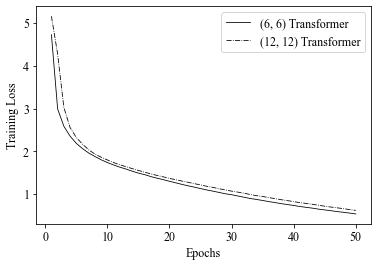
\includegraphics[width=\textwidth]{visualization/ja2pn_50E_6E_6D_vs_12E_12D.png}
    \caption{Java to Python Translation}
    \label{fig:6.1_a}
  \end{subfigure}
  ~
  \begin{subfigure}[h]{0.45\textwidth}
    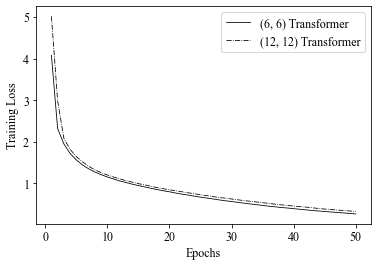
\includegraphics[width=\textwidth]{visualization/pn2ja_50E_6E_6D_vs_12E_12D.png}
    \caption{Python to Java Translation}
    \label{fig:6.1_b}
  \end{subfigure}
\caption[Training loss of the transformer model with 6 encoder layers and 6 decoder layers, and 12 encoder layers and 12 decoder layers, for 50 epochs]{Training loss of the transformer model with 6 encoder layers and 6 decoder layers, and 12 encoder layers and 12 decoder layers, for 50 epochs}
\label{fig:6.1}
\end{figure}
\noindent
The training losses of 0.5366 and 0.6188 were obtained for the transformer model with (6, 6) and (12, 12) layers, respectively, while training the models to translate from Java to Python, as shown in Figure \ref{fig:6.1_a}. In the case of Python to Java translation (Figure \ref{fig:6.1_b}), losses of 0.2692 and 0.3295 were observed for (6, 6) and (12, 12) layers, respectively.
\\\\
\textbf{CodeBERT} \\
The training losses of the models initialized with (6, 6) and (12, 12) layers of CodeBERT are shown in Figure \ref{fig:6.2}.
\begin{figure}[H]
\centering
  \begin{subfigure}[h]{0.45\textwidth}
    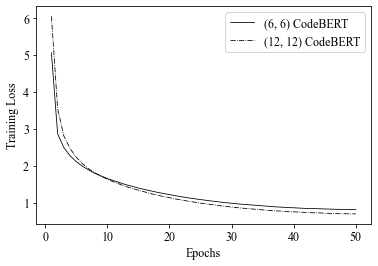
\includegraphics[width=\textwidth]{visualization/codebert_ja2pn_50E_6E_6D_vs_12E_12D.png}
    \caption{Java to Python Translation}
    \label{fig:6.2_a}
  \end{subfigure}
  ~
  \begin{subfigure}[h]{0.45\textwidth}
    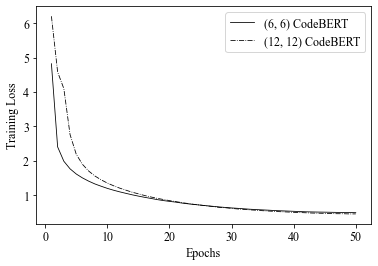
\includegraphics[width=\textwidth]{visualization/codebert_pn2ja_50E_6E_6D_vs_12E_12D.png}
    \caption{Python to Java Translation}
    \label{fig:6.2_b}
  \end{subfigure}
\caption[Training loss of the CodeBERT model with 6 encoder layers and 6 decoder layers, and 12 encoder layers and 12 decoder layers, for 50 epochs]{Training loss of the CodeBERT model with 6 encoder layers and 6 decoder layers, and 12 encoder layers and 12 decoder layers, for 50 epochs}
\label{fig:6.2}
\end{figure}
\noindent
For Java to Python translation, the losses of 0.8076 and 0.6914 were obtained for (6, 6) and (12, 12) layers, respectively; and for Python to Java translation, the losses of 0.4945 and 0.4588 were obtained, respectively.
\\\\
\textbf{Transformer vs CodeBERT} \\
Figure \ref{fig:6.3} shows the transformer and CodeBERT training losses of 0.5366 and 0.8076 for (6, 6) layers and 0.6188 and 0.6914 for (12, 12) layers when trained to translate from Java to Python; and Figure \ref{fig:6.4} shows the losses of 0.2692 and 0.4945 for (6, 6) layers and 0.3295 and 0.4588 for (12, 12) layers of the models when trained to translate from Python to Java.
\begin{figure}[H]
\centering
  \begin{subfigure}[h]{0.45\textwidth}
    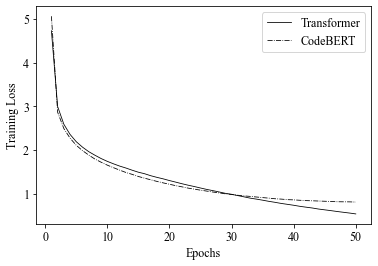
\includegraphics[width=\textwidth]{visualization/transformer_vs_codebert_ja2pn_50E_6E_6D.png}
    \caption{Training loss of the models with 6 encoder layers and 6 decoder layers}
    \label{fig:6.3_a}
  \end{subfigure}
  ~
  \begin{subfigure}[h]{0.45\textwidth}
    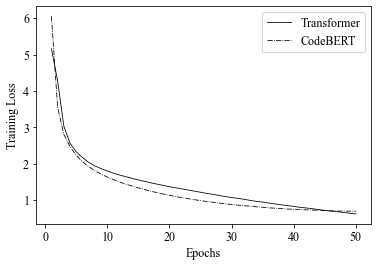
\includegraphics[width=\textwidth]{visualization/transformer_vs_codebert_ja2pn_50E_12E_12D.png}
    \caption{Training loss of the models with 12 encoder layers and 12 decoder layers}
    \label{fig:6.3_b}
  \end{subfigure}
\caption[Training loss of the transformer and CodeBERT model in Java to Python translation for 50 epochs]{Training loss of the transformer and CodeBERT model in Java to Python translation for 50 epochs}
\label{fig:6.3}
\end{figure}

\begin{figure}[H]
\centering
  \begin{subfigure}[h]{0.45\textwidth}
    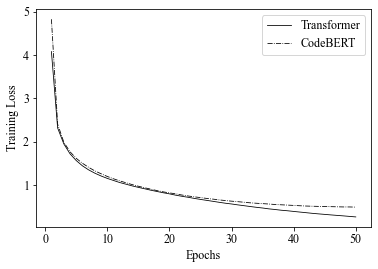
\includegraphics[width=\textwidth]{visualization/transformer_vs_codebert_pn2ja_50E_6E_6D.png}
    \caption{Training loss of the models with 6 encoder layers and 6 decoder layers}
    \label{fig:6.4_a}
  \end{subfigure}
  ~
  \begin{subfigure}[h]{0.45\textwidth}
    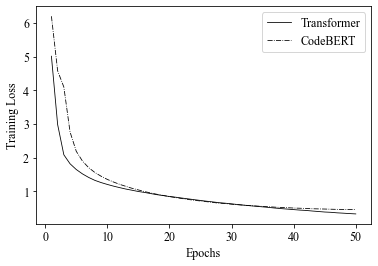
\includegraphics[width=\textwidth]{visualization/transformer_vs_codebert_pn2ja_50E_12E_12D.png}
    \caption{Training loss of the models with 12 encoder layers and 12 decoder layers}
    \label{fig:6.4_b}
  \end{subfigure}
\caption[Training loss of the transformer and CodeBERT model in Python to Java translation for 50 epochs]{Training loss of the transformer and CodeBERT model in Python to Java translation for 50 epochs}
\label{fig:6.4}
\end{figure}
\medskip
\smallskip
\textbf{Case II: 100 epochs} \\
\textbf{Transformer} \\
Figure \ref{fig:6.5_a} depicts the training loss for (6, 6) and (12, 12) transformers while training from Java to Python; the final losses are 0.1176 and 0.1461, respectively. Similarly, Figure \ref{fig:6.5_b} shows the losses of 0.0515 and 0.0697 observed in models while training in the Python to Java direction. 
\begin{figure}[H]
\centering
  \begin{subfigure}[h]{0.45\textwidth}
    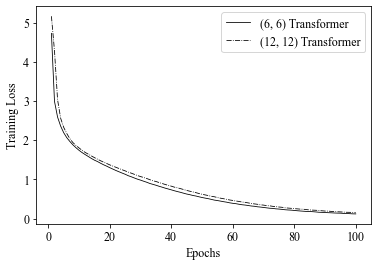
\includegraphics[width=\textwidth]{visualization/ja2pn_100E_6E_6D_vs_12E_12D.png}
    \caption{Java to Python Translation}
    \label{fig:6.5_a}
  \end{subfigure}
  ~
  \begin{subfigure}[h]{0.45\textwidth}
    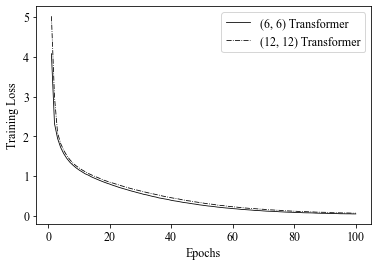
\includegraphics[width=\textwidth]{visualization/pn2ja_100E_6E_6D_vs_12E_12D.png}
    \caption{Python to Java Translation}
    \label{fig:6.5_b}
  \end{subfigure}
\caption[Training loss of the transformer model with 6 encoder layers and 6 decoder layers, and 12 encoder layers and 12 decoder layers, for 100 epochs]{Training loss of the transformer model with 6 encoder layers and 6 decoder layers, and 12 encoder layers and 12 decoder layers, for 100 epochs}
\label{fig:6.5}
\end{figure}
\medskip
\smallskip
\textbf{CodeBERT} \\
Figure \ref{fig:6.6} shows the loss for (6, 6) and (12, 12) CodeBERT models trained in Java to Python direction; the losses are 0.3088 and 0.5233, respectively. In Java to Python direction, the losses observed are 0.1381 and 0.1575, respectively.
\begin{figure}[H]
\centering
  \begin{subfigure}[h]{0.45\textwidth}
    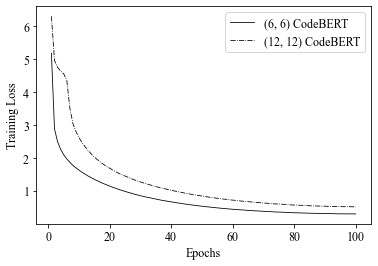
\includegraphics[width=\textwidth]{visualization/codebert_ja2pn_100E_6E_6D_vs_12E_12D.png}
    \caption{Java to Python Translation}
    \label{fig:6.6_a}
  \end{subfigure}
  ~
  \begin{subfigure}[h]{0.45\textwidth}
    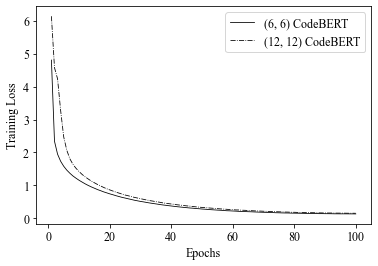
\includegraphics[width=\textwidth]{visualization/codebert_pn2ja_100E_6E_6D_vs_12E_12D.png}
    \caption{Python to Java Translation}
    \label{fig:6.6_b}
  \end{subfigure}
\caption[Training loss of the CodeBERT model with 6 encoder layers and 6 decoder layers, and 12 encoder layers and 12 decoder layers, for 50 epochs]{Training loss of the CodeBERT model with 6 encoder layers and 6 decoder layers, and 12 encoder layers and 12 decoder layers, for 50 epochs}
\label{fig:6.6}
\end{figure}
\medskip
\smallskip
\textbf{Transformer vs CodeBERT}\\
The training losses of (6, 6) and (12, 12) layers transformer and CodeBERT models in Java to Python translation direction are shown in Figure \ref{fig:6.7}. For (6, 6) layers the loss at the end of epoch for the transformer model is 0.1176 and for the CodeBERT model is 0.3088. For (12, 12) layers the loss for the tranformer model is 0.1461 and the CodeBERT model is 0.5233.
\begin{figure}[H]
\centering
  \begin{subfigure}[h]{0.45\textwidth}
    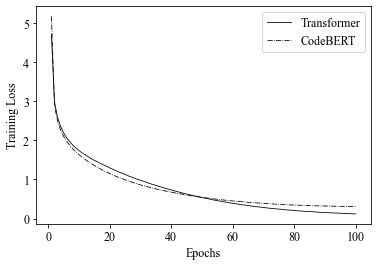
\includegraphics[width=\textwidth]{visualization/transformer_vs_codebert_ja2pn_100E_6E_6D.png}
    \caption{Training loss of the models with 6 encoder layers and 6 decoder layers}
    \label{fig:6.7_a}
  \end{subfigure}
  ~
  \begin{subfigure}[h]{0.45\textwidth}
    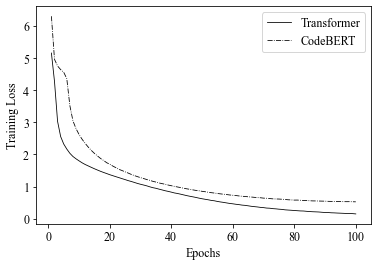
\includegraphics[width=\textwidth]{visualization/transformer_vs_codebert_ja2pn_100E_12E_12D.png}
    \caption{Training loss of the models with 12 encoder layers and 12 decoder layers}
    \label{fig:6.7_b}
  \end{subfigure}
\caption[Training loss of the transformer and CodeBERT model in Java to Python translation for 100 epochs]{Training loss of the transformer and CodeBERT model in Java to Python translation for 100 epochs}
\label{fig:6.7}
\end{figure}
Similarly, the training losses for the transformer and CodeBERT models in Python to Java translation direction are show in Figure \ref{fig:6.8}. The transformer and CodeBERT model with (6, 6) layers have training loss 0.0514, 0.1381 respectively, and with (12, 12) layers have 0.0697, 0.1575, respectively.
\begin{figure}[H]
\centering
  \begin{subfigure}[h]{0.45\textwidth}
    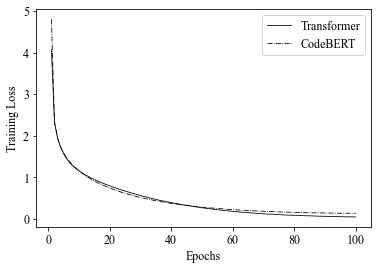
\includegraphics[width=\textwidth]{visualization/transformer_vs_codebert_pn2ja_100E_6E_6D.png}
    \caption{Training loss of the models with 6 encoder layers and 6 decoder layers}
    \label{fig:6.8_a}
  \end{subfigure}
  ~
  \begin{subfigure}[h]{0.45\textwidth}
    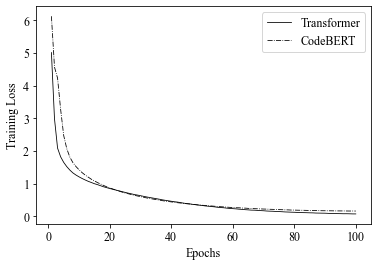
\includegraphics[width=\textwidth]{visualization/transformer_vs_codebert_pn2ja_100E_12E_12D.png}
    \caption{Training loss of the models with 12 encoder layers and 12 decoder layers}
    \label{fig:6.8_b}
  \end{subfigure}
\caption[Training loss of the transformer and CodeBERT model in Python to Java translation for 100 epochs]{Training loss of the transformer and CodeBERT model in Python to Java translation for 100 epochs}
\label{fig:6.8}
\end{figure}
%\vspace*{-32pt}
\section{Results}
The BLEU and CodeBLEU scores of the transformer and CodeBERT models obtained for 627 testing samples are shown in Table \ref{table:6.1} (Java to Python) and Table \ref{table:6.2} (Python to Java).
\begin{table}[H]
\centering
\def\arraystretch{1.25}
\caption{BLEU, CodeBLEU, WNM, SM, and DM scores for Java to Python translation}
\label{table:6.1}
\begin{tabular}{|P{1.15cm}|P{1.15cm}|c|c|c|c|c|c|c|} \hline
\textbf{No. of epochs} & \textbf{No. of layers} & \textbf{Model} & \textbf{BLEU} & \textbf{CodeBLEU} & \textbf{WNM} & \textbf{SM} & \textbf{DM}\\ \hline
\multirow{4}{*}{50} & \multirow{2}{*}{6} & Transformer & \textbf{0.2812} & \textbf{0.2802} & \textbf{0.2828} & 0.3137 & 0.2430 \\ \cline{3-8}
			      & 			      & CodeBERT & 0.1294 & 0.2109 & 0.1321 & \textbf{0.3491} & 0.2334 \\ \cline{2-8}
 			      & \multirow{2}{*}{12} & Transformer & 0.2627 & 0.2724 & 0.2642 & 0.3227 & 0.2400 \\ \cline{3-8}
			      & 			      & CodeBERT & 0.0977 & 0.1897 & 0.1028 & 0.3439 & 0.2152 \\ \hline
\multirow{4}{*}{100} & \multirow{2}{*}{6} & Transformer & 0.2659 & 0.2733 & 0.2683 & 0.3097 & \textbf{0.2492} \\ \cline{3-8}
			      & 			      & CodeBERT & 0.1512 & 0.2233 & 0.1539 & 0.3485 & 0.2401 \\ \cline{2-8}
 			      & \multirow{2}{*}{12} & Transformer & 0.2519 & 0.2656 & 0.2536 & 0.3154 & 0.2415 \\ \cline{3-8}
			      & 			      & CodeBERT & 0.1067 & 0.1745 & 0.1092 & 0.3063 & 0.1760 \\ \hline
\end{tabular}
\end{table}

\begin{table}[H]
\centering
\def\arraystretch{1.25}
\caption{BLEU, CodeBLEU, WNM, SM, and DM scores for Python to Java translation}
\label{table:6.2}
\begin{tabular}{|P{1.15cm}|P{1.15cm}|c|c|c|c|c|c|c|} \hline
\textbf{No. of epochs} & \textbf{No. of layers} & \textbf{Model} & \textbf{BLEU} & \textbf{CodeBLEU} & \textbf{WNM} & \textbf{SM} & \textbf{DM}\\ \hline
\multirow{4}{*}{50} & \multirow{2}{*}{6} & Transformer & 0.3883 & 0.4016 & 0.3990 & 0.4715 & 0.3434 \\ \cline{3-8}
			      & 			      & CodeBERT & 0.2747 & 0.3495 & 0.3006 & 0.4857 & 0.3234 \\ \cline{2-8}
 			      & \multirow{2}{*}{12} & Transformer & 0.3633 & 0.3841 & 0.3744 & 0.4591 & 0.3358 \\ \cline{3-8}
			      & 			      & CodeBERT & 0.2580 & 0.3299 & 0.2770 & 0.4644 & 0.3112 \\ \hline
\multirow{4}{*}{100} & \multirow{2}{*}{6} & Transformer & \textbf{0.3891} & \textbf{0.4018} & \textbf{0.4012} & 0.4613 & \textbf{0.3526} \\ \cline{3-8}
			      & 			      & CodeBERT & 0.2938 & 0.3727 & 0.3203 & \textbf{0.5172} & 0.3458 \\ \cline{2-8}
 			      & \multirow{2}{*}{12} & Transformer & 0.3652 & 0.3837 & 0.3778 & 0.4461 & 0.3434 \\ \cline{3-8}
			      & 			      & CodeBERT & 0.2936 & 0.3697 & 0.3183 & 0.5120 & 0.3424 \\ \hline
\end{tabular}
\end{table}

\section{Analysis}
In order to choose the appropriate model for program translation, the study evaluates the BLEU and CodeBLEU scores of the CodeBERT and the transformer models. The study uses trained models to translate programs from the test dataset and compute BLEU and CodeBLEU scores. It determines whether the Python to Java program translation models have equivalent BLEU and CodeBLEU scores to the Java to Python program translation models.
\\\\
The transformer model with 6 layers has a lower training loss than the model with 12 layers over a period of 50 epochs. Both the 6-layer Java to Python transformer translation model and the 6-layer Python to Java transformer translation model have losses of 0.5366 and 0.2692, respectively. In the case of the CodeBERT models trained for 50 epochs, the 12-layer models exhibit less loss than the 6-layer models. The loss for the 12-layer Java to Python CodeBERT model is 0.6914, and the loss for the Python to Java CodeBERT model is 0.4588. In comparison to CodeBERT models with 6 layers, transformer models with 6 layers produce lower training loss. The 6-layer transformer model has a loss of 0.5366 and 0.2692 when training from Java to Python and Python to Java, respectively. The 12-layer transformer also performs better than the 12-layer CodeBERT in terms of training loss, with losses of 0.3295 and 0.6188 when training from Python to Java and Java to Python, respectively. Even for 100 epochs, the 6-layer transformer models have less training loss than the 12-layer transformer models. Likewise, 6-layer CodeBERT models show less loss than 12-layer CodeBERT models after 100 training epochs. For 100 training epochs, the CodeBERT models also suffer from high training loss in comparison to the transformer models.
\\\\
The results shown in Table 6.1 demonstrate that the transformer model with 6 encoder and 6 decoder layers, trained for 50 epochs to translate from Java to Python, received the highest BLEU and CodeBLEU scores, with values of 0.2812 and 0.2802, respectively. According to the results shown in Table 6.2, the transformer model, trained for 100 epochs to translate from Python to Java, achieved the highest BLEU and CodeBLEU scores, respectively, of 0.3891 and 0.4018. This model also has 6 encoder and 6 decoder layers. Additionally, the results demonstrate that Python to Java translation models have higher BLEU and CodeBLEU scores than Java to Python translation models.
\\\\
In this study, the transformer models have performed better than the CodeBERT models in terms of BLEU and CodeBLEU scores. In addition to this, the transformer models have achieved higher WNM, and DM scores than the CodeBERT models. However, the SM scores of the transformer models are lower than those of the CodeBERT models.







\chapter{Conclusion}
\section{Conclusion}
The purpose of this study was to compare the transformer and the CodeBERT model on program translation tasks. The study used a 3133 Java-Python parallel program dataset to translate the programs written in the source language to the target language. 80\% (2506) of the data was used to train and 20\% (672) of the data was used to test the transformer and the CodeBERT models. To be able to translate the programs, the study followed the following steps: data preprocessing, model training, inference, and data postprocessing.
\\\\
Based on the BLEU and CodeBLEU scores of the models trained for different epochs, it can be concluded that the transformer models performed better than the CodeBERT models on the test dataset used in the study. For the Java to Python program translation task, the transformer model with 6 encoder and 6 decoder layers trained for 50 epochs achieved the highest BLEU and Code BLEU scores, of 0.2812 and 0.2802, respectively. Similarly, for the Python to Java program translation task, the transformer model with 6 encoder and 6 decoder layers trained for 100 epochs received the highest BLEU and CodeBLEU scores, with values of 0.3891 and 0.4018, respectively. Furthermore, the scores of Java to Python translation models differ from those of Python to Java translation models.

\section{Limitations}
The study on program translation has the following limitations:
\begin{itemize}[nosep]
\item The autoregressive model pretrained on codes exists. However, the study focused on exploiting the public CodeBERT checkpoint to initialize the encoder and the decoder of the encoder-decoder model.
\item The parallel corpora of other programming languages, such as Java-C++, Java-C\#, PHP-Java, etc., are also available, but the study used only the Java-Python corpus to train and evaluate the models.
\item Despite the availability of evaluation metrics like computational accuracy, the dissertation has focused on using BLEU and CodeBLEU scores, which are the most extensively used evaluation metrics for assessing the performance of the translation models.
\end{itemize}

\section{Future Recommendations}
The study used the CodeBERT block on both the encoder and decoder side of the translation model with shared weights. It is possible to use an autoregressive model on the decoder side. Additionally, due to resource constraints, the experiment was run on a small set of data. It would have been good if all of the datasets were used to train the models.

\newpage
\addcontentsline{toc}{chapter}{References}
\printbibliography[title={References}]

\appendix

\appendixtocstyle
\chapter{Sample Dataset}
\textbf{Sample 1:}\\ % java-python_GeeksForGeeks_4023_A_1
\textbf{Java Program}\\
\vspace*{-\baselineskip}
\begin{Verbatim}[frame=single]
// Java implementation to find  
// the sum of the given series 
import java.io.*; 
  
class GfG { 
      
// function to find the sum 
// of the given series 
static int sumOfTheSeries(int n) 
{ 
    // required sum 
    return (n * (n + 1) / 2) * 
            (2 * n + 1) / 3; 
} 
      
  
// Driver program to test above 
public static void main (String[] args)  
{ 
    int n = 5; 
      
    System.out.println("Sum = "+  
                sumOfTheSeries(n)); 
  
} 
  
} 
  
// This code is contributed by Gitanjali. 
\end{Verbatim}
\textbf{Python Program} \\
\vspace*{-\baselineskip}
\begin{Verbatim}[frame=single]
# Python3 implementation to find 
# the sum of the given series 
  
# functionn to find the sum 
# of the given series 
def sumOfTheSeries( n ): 
      
    # required sum 
    return int((n * (n + 1) / 2) *
            (2 * n + 1) / 3) 
              
# Driver program to test above 
n = 5
print("Sum =", sumOfTheSeries(n)) 
  
# This code is contributed by "Sharad_Bhardwaj". 
\end{Verbatim}
\newpage
\textbf{Sample 2:} \\ % java-python_ProjectEuler_p007_A_30
\textbf{Java Program} \\
\vspace*{-\baselineskip}
\begin{Verbatim}[frame=single, breaklines=true, breakanywhere=true]
/* 
 * Solution to Project Euler problem 7
 * Copyright (c) Project Nayuki. All rights reserved.
 * 
 * https://www.nayuki.io/page/project-euler-solutions
 * https://github.com/nayuki/Project-Euler-solutions
 */


public final class p007 implements EulerSolution {
	
	public static void main(String[] args) {
		System.out.println(new p007().run());
	}
	
	
	/* 
	 * Computers are fast, so we can implement this solution by testing each number
	 * individually for primeness, instead of using the more efficient sieve of Eratosthenes.
	 */
	public String run() {
		for (int i = 2, count = 0; ; i++) {
			if (Library.isPrime(i)) {
				count++;
				if (count == 10001)
					return Integer.toString(i);
			}
		}
	}
	
}
\end{Verbatim}
\textbf{Python Program} \\
\vspace*{-\baselineskip}
\begin{Verbatim}[frame=single, breaklines=true, breakanywhere=true]
# 
# Solution to Project Euler problem 7
# Copyright (c) Project Nayuki. All rights reserved.
# 
# https://www.nayuki.io/page/project-euler-solutions
# https://github.com/nayuki/Project-Euler-solutions
# 

import eulerlib, itertools


# Computers are fast, so we can implement this solution by testing each number
# individually for primeness, instead of using the more efficient sieve of Eratosthenes.
# 
# The algorithm starts with an infinite stream of incrementing integers starting at 2,
# filters them to keep only the prime numbers, drops the first 10000 items,
# and finally returns the first item thereafter.
def compute():
	ans = next(itertools.islice(filter(eulerlib.is_prime, itertools.count(2)), 10000, None))
	return str(ans)


if __name__ == "__main__":
	print(compute())
\end{Verbatim}


\chapter{Example Translation}
A single Java-Python parallel program from the test dataset is:\\
\textbf{Java Program}\\
\vspace*{-\baselineskip}
\begin{Verbatim}[frame=single]
// Java program to find sum of all elements 
// upto nth row in Pascal triangle. 
import java.io.*; 
  
class GFG { 
  
    // Function to find sum of aal elements 
    // upto nth row. 
    static long calculateSum(int n) 
    { 
  
        // Initialize sum with 0 
        long sum = 0; 
  
        // Loop to calculate power of 2 
        // upto n and add them 
        for (int row = 0; row < n; row++) { 
            sum = sum + (1 << row); 
        } 
  
        return sum; 
    } 
  
    // Driver code 
    public static void main(String[] args) 
    { 
        int n = 10; 
        System.out.println("Sum of all elements:"
                           + calculateSum(n)); 
    } 
}  
\end{Verbatim}
\textbf{Python Program}\\
\vspace*{-\baselineskip}
\begin{Verbatim}[frame=single]
# Python program to find sum of all elements 
# upto nth row in Pascal triangle. 
  
# Function to find sum of aal elements 
# upto nth row. 
def calculateSum(n) : 
          
    # Initialize sum with 0 
    sum = 0
      
    # Loop to calculate power of 2 
    # upto n and add them 
    for row in range(n): 
        sum = sum + (1 << row) 
  
    return sum
      
# Driver code     
n = 10
print("Sum of all elements:", calculateSum(n)) 
\end{Verbatim}
\newpage
The following is an illustration of the outputs generated by the steps in the translation process: \\\\
\textbf{Case I: Java to Python translation using the transformer model with 6 encoder and 6 decoder layers trained for 50 epochs } 
\begin{enumerate}[topsep = 0pt, label = \roman*.]
\item Pretokenization \\
%\vspace*{-\baselineskip}
\vspace*{-\baselineskip}
\begin{Verbatim}[frame=single, breaklines=true, breakanywhere=true]
import java . io . * ; class GFG { static long calculateSum ( int n ) { long sum = 0 ; for ( int row = 0 ; row < n ; row ++ ) { sum = sum + ( 1 << row ) ; } return sum ; } public static void main ( String [ ] args ) { int n = 10 ; System . out . println ( "Sum of all elements:" + calculateSum ( n ) ) ; } }
\end{Verbatim}

\item Tokenization \\
\vspace*{-\baselineskip}
\begin{Verbatim}[frame=single, breaklines=true, breakanywhere=true]
import java . io . * ; class GFG { static long calculateSum ( int n ) { long sum = 0 ; for ( int row = 0 ; row < n ; row ++ ) { sum = sum + ( 1 << row ) ; } return sum ; } public static void main ( String [ ] args ) { int n = 10 ; System . out . println ( "Sum of all elements:" + calculateSum ( n ) ) ; } 
\end{Verbatim}

\item Translation \\
\vspace*{-\baselineskip}
\begin{Verbatim}[frame=single, breaklines=true, breakanywhere=true]
 def calculateSum ( n ) : NEWLINE INDENT sum = 0 ; NEWLINE for i in range ( n ) : NEWLINE INDENTINDENT sum = sum + ( 1 << i ) ; NEWLINE DEDENT return sum ; NEWLINE DEDENT n = 10 ; NEWLINE print ( "Sum of all is" , calculateSum ( n ) ) NEWLINE NL ENDMARKER 
\end{Verbatim}

\item Data Postprocessing \\
\vspace*{-\baselineskip}
\begin{Verbatim}[frame=single, breaklines=true, breakanywhere=true]
def calculateSum(n):
 sum=0;
for i in range(n):
 sum=sum+(1<<i);
return sum;
n=10;
print("Sum of all is",calculateSum(n))
# Created by pyminifier (https://github.com/liftoff/pyminifier)
\end{Verbatim}
\end{enumerate}

\textbf{Case II: Java to Python translation using the CodeBERT model with 6 encoder and 6 decoder layers trained for 100 epochs }
\begin{enumerate}[topsep = 0pt, label = \roman*.]
\item Pretokenization \\
\vspace*{-\baselineskip}
\begin{Verbatim}[frame=single, breaklines=true, breakanywhere=true]
import java.io. * ; class GFG { static long calculateSum(int n) { long sum = 0; for(int row = 0; row < n; row ++ ) { sum = sum + (1 << row); } return sum; } public static void main(String[]args) { int n = 10; System.out.println("Sum of all elements:" + calculateSum(n)); } }
\end{Verbatim}

\item Tokenization \\
\vspace*{-\baselineskip}
\begin{Verbatim}[frame=single, breaklines=true, breakanywhere=true]
import Ġjava . io . Ġ* Ġ; Ġclass ĠG FG Ġ{ Ġstatic Ġlong Ġcalculate Sum ( int Ġn ) Ġ{ Ġlong Ġsum Ġ= Ġ0 ; Ġfor ( int Ġrow Ġ= Ġ0 ; Ġrow Ġ< Ġn ; Ġrow Ġ++ Ġ) Ġ{ Ġsum Ġ= Ġsum Ġ+ Ġ( 1 Ġ<< Ġrow ); Ġ} Ġreturn Ġsum ; Ġ} Ġpublic Ġstatic Ġvoid Ġmain ( String [] args ) Ġ{ Ġint Ġn Ġ= Ġ10 ; ĠSystem . out . println (" Sum Ġof Ġall Ġelements :" Ġ+ Ġcalculate Sum ( n )); Ġ} Ġ}
\end{Verbatim}

\item Translation \\
\vspace*{-\baselineskip}
\begin{Verbatim}[frame=single, breaklines=true, breakanywhere=true]
def calculateSum(n): NEWLINE INDENT sum=0 NEWLINE for i in range(0,n+1): NEWline INDENTINDENT sum+=i NEWLINE DEDENT  return sum NEWLINE d=sum-1 NEWLINE print("Sum of triangular",calculateSum(num)) NEWLINE NL ENDMARKER
\end{Verbatim}

\item Data Postprocessing \\
\vspace*{-\baselineskip}
\begin{Verbatim}[frame=single, breaklines=true, breakanywhere=true]
def calculateSum(n):
     sum=0
for i in range(0,n+1):
         sum+=i
 return sum
d=sum-1
print("Sum of triangular",calculateSum(num))
\end{Verbatim}
\end{enumerate}

\textbf{Case III: Python to Java translation using the transformer model with 6 encoder and 6 decoder layers trained for 100 epochs }
\begin{enumerate}[topsep = 0pt, label = \roman*.]
\item Data Cleaning \\
\vspace*{-\baselineskip}
\begin{Verbatim}[frame=single, breaklines=true, breakanywhere=true]
def calculateSum(n):
 sum=0
 for row in range(n):
  sum=sum+(1<<row)
 return sum
n=10
print("Sum of all elements:",calculateSum(n))
# Created by pyminifier (https://github.com/liftoff/pyminifier)
\end{Verbatim}

\item Pretokenization \\
\vspace*{-\baselineskip}
\begin{Verbatim}[frame=single, breaklines=true, breakanywhere=true]
def calculateSum ( n ) : NEWLINE INDENT sum = 0 NEWLINE for row in range ( n ) : NEWLINE INDENTINDENT sum = sum + ( 1 << row ) NEWLINE DEDENT return sum NEWLINE DEDENT n = 10 NEWLINE print ( "Sum of all elements:" , calculateSum ( n ) ) NEWLINE NL ENDMARKER
\end{Verbatim}

\item Tokenization \\
\vspace*{-\baselineskip}
\begin{Verbatim}[frame=single, breaklines=true, breakanywhere=true]
def calculateSum ( n ) : NEWLINE INDENT sum = 0 NEWLINE for row in range ( n ) : NEWLINE INDENTINDENT sum = sum + ( 1 << row ) NEWLINE DEDENT return sum NEWLINE DEDENT n = 10 NEWLINE print ( "Sum of all elements:" , calculateSum ( n ) ) NEWLINE NL 
\end{Verbatim}
\newpage
\item Translation \\
\vspace*{-\baselineskip}
\begin{Verbatim}[frame=single, breaklines=true, breakanywhere=true]
import java . io . * ; class GFG { static long calculateSum ( int n ) { long sum = 0 ; for ( int i = 0 ; i < n ; i ++ ) { sum = sum + ( 1 << i ) ; } return sum ; } public static void main ( String [ ] args
\end{Verbatim}

\item Data Postprocessing \\
\vspace*{-\baselineskip}
\begin{Verbatim}[frame=single, breaklines=true, breakanywhere=true]
import java.io. * ;
class GFG {
    static long calculateSum(int n) {
        long sum = 0;
        for(int i = 0;
        i < n;
        i ++ ) {
            sum = sum + (1 << i);
            
        }
        return sum;
        
    }
    public static void main(String[]args
\end{Verbatim}
\end{enumerate}

\textbf{Case IV: Python to Java translation using the CodeBERT model with 6 encoder and 6 decoder layers trained for 100 epochs }
\begin{enumerate}[topsep = 0pt, label = \roman*.]
\item Data Cleaning \\
\vspace*{-\baselineskip}
\begin{Verbatim}[frame=single, breaklines=true, breakanywhere=true]
def calculateSum(n):
 sum=0
 for row in range(n):
  sum=sum+(1<<row)
 return sum
n=10
print("Sum of all elements:",calculateSum(n))
# Created by pyminifier (https://github.com/liftoff/pyminifier)
\end{Verbatim}

\item Pretokenization \\
\vspace*{-\baselineskip}
\begin{Verbatim}[frame=single, breaklines=true, breakanywhere=true]
def calculateSum(n): NEWLINE INDENT sum=0 NEWLINE for row in range(n): NEWLINE INDENTINDENT sum=sum+(1<<row) NEWLINE DEDENT  return sum NEWLINE DEDENT n=10 NEWLINE print("Sum of all elements:",calculateSum(n)) NEWLINE NL ENDMARKER
\end{Verbatim}

\item Tokenization \\
\vspace*{-\baselineskip}
\begin{Verbatim}[frame=single, breaklines=true, breakanywhere=true]
def Ġcalculate Sum ( n ): ĠNEW LINE ĠIND ENT Ġsum = 0 ĠNEW LINE Ġfor Ġrow Ġin Ġrange ( n ): ĠNEW LINE ĠIND ENT IND ENT Ġsum = sum +( 1 << row ) ĠNEW LINE ĠD ED ENT Ġ Ġreturn Ġsum ĠNEW LINE ĠD ED ENT Ġn = 10 ĠNEW LINE Ġprint (" Sum Ġof Ġall Ġelements : ", cal cul ate Sum ( n )) ĠNEW LINE ĠNL ĠEND M ARK ER
\end{Verbatim}

\item Translation \\
\vspace*{-\baselineskip}
\begin{Verbatim}[frame=single, breaklines=true, breakanywhere=true]
import java.io. * ; class GFG { static long calculateSum(int n) { long sum = 0; for(int i = 0, sum = 1; i < n; i ++ )sum += (1 << i); return sum; } public static void main(String[]args) { int n = 10; System.out.println("Sum of the series : " + calculateSum of n + " = " + sum(n)); } }
\end{Verbatim}

\item Data Postprocessing \\
\vspace*{-\baselineskip}
\begin{Verbatim}[frame=single, breaklines=true, breakanywhere=true]
import java.io. * ;
class GFG {
    static long calculateSum(int n) {
        long sum = 0;
        for(int i = 0, sum = 1;
        i < n;
        i ++ )sum += (1 << i);
        return sum;
        
    }
    public static void main(String[]args) {
        int n = 10;
        System.out.println("Sum of the series : " + calculateSum of n + " = " + sum(n));
        
    }
}
\end{Verbatim}
\end{enumerate}



\end{document}